\documentclass[10pt, a4paper]{article}
\usepackage[utf8]{inputenc}
\usepackage{verbatim}
\usepackage{mathtools}
\usepackage{float}
%\usepackage{graphicx}
\usepackage[]{algorithm2e}
\usepackage{amssymb}
\usepackage[conEntregas]{caratula}

\usepackage[square,sort,comma,numbers]{natbib}\usepackage{graphicx}
%agregados por anto los proximos, no agregar subcaption xq los bloquea:
\usepackage{enumitem} 
\usepackage{subfigure}

\begin{document}

\titulo{TP 3: Demosaicing}

\fecha{13/11/2014}

\materia{M\'etodos Numericos}
%\grupo{Grupo ?}

\integrante{Dellanzo, Claudia Antonella}{019/13}{anto\_tbdt@hotmail.com}
\integrante{De Rocco, Federico}{403/13}{fede.183@hotmail.com}
\integrante{Tallar, Nicol\'as}{218/13}{nicot.sanlorenzo@hotmail.com}
% Pongan cuantos integrantes quieran

\maketitle

\section{Introducci\'on}

El objetivo de este trabajo pr\'actico es el de seguir implementando nuevas aplicaciones de los temas vistos en clase y seguir viendo como se pueden utilizar estos para solucionar diferentes problemas. En este trabajo, nos centramos en la utilizaci\'on de la interpolaci\'on para poder resolver el problema de demosaicing, el cual esta causado porque las c\'amaras digitales, al tomar las im\'agenes, no toman en cada uno de sus sensores todos los colores, s\'olo toman uno de ellos. Esto causa que en muchos casos la im\'agen obtenida sea de la siguiente forma:

\begin{table}[h]
\centering
\begin{tabular}{|c | c | c | c |
}
\hline
B & G & B & \ldots \\
\hline
G & R & G & \ldots \\
\hline
B & G & B & \ldots \\
\hline
$\vdots$ & $\vdots$ & $\vdots$ & $\ddots$ \\
\hline
\end{tabular}
\end{table}

A la forma en que estan organizados los sensores y que color capturan en cada posici\'on se le llama el bayer array, aunque no siempre esta organizado tal como mostramos anteriormente, debido a que los sensores pueden estar organizados de otra manera. 
Igualmente, nosotros vamos a tomar que las fotos con las que trabajamos fueron tomadas por una c\'amara con los sensores organizados tal como se muestra en el ejemplo. Entonces el objetivo de este trabajo es realizar diferentes m\'etodos para pasar de una im\'agen obtenida de esta forma a una que en cada pixel tenga los valores correctos (o aproximadamente correctos), para cada uno de los colores. Uno de los principales m\'etodos para la realizaci\'on de esto es la utilizaci\'on de la interpolaci\'on para asi poder realizar diferentes estimaciones sobre los valores que debe tener los colores de un pixel y juntar estos mediante diferentes maneras, de forma tal de obtener un mejor resultado. Por lo que en este trabajo nos vamos a dedicar a implementar diferentes versiones de esta y luego analizar cuales de ellas son mejores, en termino de calidad y tiempo.

\section{Bayer}

Para poder realizar los algoritmos de demosaicing, deberemos trabajar con una imagen en formato \textit{Bayer}, en el cual cada pixel posee 2 canales en 0 y el restante con un valor determinado. Para realizar el mismo seguiremos el formato presentado en el enunciado (el cual contiene en las filas pares solo azul y verde, y en las impares rojo y verde). 

Para realizar el mismo tomamos la imagen y vamos recorri\'endola, anulando en cada paso los canales correspondientes. Si nos encontramos en una fila y columnas impar, deberemos anular el canal verde y el azul, si es fila impar y columna par deberemos anular el canal rojo y azul, si es fila y columna par deberemos anular el canal rojo y azul y, por \'ultimo, si es fila par y columna impar deberemos anular el canal rojo y verde. De esta forma pasamos la imagen original de RGB a Bayer Color filter Array (CFA), con la que trabajaremos en todos los algoritmos que se popondr\'an en este informe.

\section{Vecino m\'as cercano}

Este es un algoritmo de demosaicing que consiste en obtener el valor buscado de un canal de un p\'ixel de otro p\'ixel pr\'oximo a este. La forma en la que esto se resolvi\'o fue recorriendo el filter array Bayer y, sabiendo que color posee cada p\'ixel por su ubicaci\'on, hacer lo siguiente por cada uno:
\ \\
\begin{algorithm}[H]

\ \\
$imagen[i,j,rojo]=imagen[i,j-1,rojo]$\;
$imagen[i,j,azul]=imagen[i-1,j,azul]$\;
\caption{Caso en que estemos en un p\'ixel verde de fila con rojos(Posici\'on i, j de la matriz)}
\end{algorithm} 
\ \\
\ \\
\begin{algorithm}[H]

\ \\
$imagen[i,j,rojo]=imagen[i-1,j,rojo]$\;
$imagen[i,j,azul]=imagen[i,j-1,azul]$\;
\caption{Caso en que estemos en un p\'ixel verde de fila con azules(Posici\'on i, j de la matriz)}
\end{algorithm} 
\ \\
\ \\
\begin{algorithm}[H]

\ \\
$imagen[i,j,azul]=imagen[i-1,j-1,azul]$\;
$imagen[i,j,verde]=imagen[i,j-1,verde]$\;
\caption{Caso en que estemos en un p\'ixel rojo(Posici\'on i, j de la matriz)}
\end{algorithm} 
\ \\
\ \\
\begin{algorithm}[H]

\ \\
$imagen[i,j,rojo]=imagen[i-1,j-1,rojo]$\;
$imagen[i,j,verde]=imagen[i,j-1,verde]$\;
\caption{Caso en que estemos en un p\'ixel azul(Posici\'on i, j de la matriz)}
\end{algorithm} 
\ \\

Este algoritmo no toma en cuenta los bordes, los cuales son recortados. Adem\'as, la matriz es recorrida sin tomarlos en cuenta. La elecci\'on de estos puntos como vecinos se debe a que, con cada uno de ellos, no se requiere tomar en cuenta ning\'un caso borde. Esto se traduce a un caso donde el vecino a buscar no exista. 
Para recorrer la matriz se usaran cuatro ciclos dobles. Cada uno se encargar\'a de recorrer la matriz respecto a las posiciones de cada uno de los cuatro casos anteriormente descriptos. Esto sirve principalmente para evitar el uso de if los cuales ralentizan el algoritmo. En cambio, con los ciclos que elegimos, se har\'a el mismo camino sin la necesidad de usar condicionales.

%Falta completar
\section{Interpolaci\'on bilineal}

Este m\'etodo consiste en utilizar interpolaciones lineales para poder adquirir el valor del canal de un p\'ixel. Para esto se definir\'a una funci\'on que se encargar\'a de realizar la interpolaci\'on con el polinomio de Lagrange. Solo se realizar\'an interpolaciones usando dos puntos, es decir seleccionando los canales de un color de dos p\'ixeles. El siguiente es el algoritmo utilizado para interpolar:

\ \\
\begin{algorithm}[H]
\ \\
\textbf{IN} x0 y x1 son los puntos a interpolar(Enteros)\;
\textbf{IN} y0 y y1 son los valores del canal en cuesti\'on en esos puntos(Float)\;
\textbf{IN} x es la posici\'on del canal del p\'ixel que se desea completar\;
$resultado=y1*(x-x0)/(x1-x0)+(y0*(x-x1)/(x0-x1))$\;
\caption{Algoritmo de interpolaci\'on lineal}
\end{algorithm} 
\ \\

Se tomar\'a como x0 y x1 como la posici\'on de la matriz en la que se encuentran los p\'ixeles de los que tomaremos el color de alg\'un canal. Para yo e y1 nos limitaremos a utilizar el valor del canal que es buscado en esos puntos. El x ser\'a el que referencia al canal del p\'ixel buscado. Esto lo usaremos para interpolar los canales rojo y azul de los p\'ixeles verdes, el azul en los rojos y el rojo en los azules. Para el caso de obtener el color verde de los rojos y azules, hicimos algo m\'as simple y utilizamos el algoritmo que figura en [1] que es simplemente tomar el promedio de los cuatro canales verdes de los p\'ixeles de alrededor. Este \'ultimo nos ahorra tener que hacer otra interpolaci\'on con esos cuatro p\'ixeles. 

Para el algoritmo recorreremos cada pixel de la matriz y, seg\'un en que caso estemos, realizaremos alguno de los siguientes pasos, en donde \textit{Posicion del Punto} nos devuelve, dada una posici\'on \textit{i, j}, el lugar que ocupa en el array que representa a la imagen: 

\ \\
\begin{algorithm}[H]
//Suponiendo que estamos en la posici\'on \textit{i, j} de la imagen
x0 = Posicion del punto $(i-1,j)$\;
x1 = Posicion del punto $(i+1,j)$\;
y0 = Canal azul de la posicion $(i-1,j)$\;
y1 = Canal azul de la posicion $(i+1,j)$\;
x = Posicion del punto $(i,j)$\;

Canal azul de la posicion (i,j) = Interpolacion lineal de x0, x1, y0, y1, x\;

x0 = Posicion del punto $(i,j-1)$\;
x1 = Posicion del punto $(i,j+1)$\;
y0 = Canal azul de la posicion $(i,j-1)$\;
y1 = Canal azul de la posicion $(i,j+1)$\;
x = Posicion del punto $(i,j)$\;

Canal azul de la posicion $(i,j)$ = Interpolacion lineal de x0, x1, y0, y1, x

\caption{Caso en que estemos en un p\'ixel verde de fila con rojos}
\end{algorithm} 
\ \\
\ \\
\begin{algorithm}[H]
//Suponiendo que estamos en la posici\'on \textit{i, j} de la imagen
x0 = Posicion del punto $(i,j-1)$\;
x1 = Posicion del punto $(i,j+1)$\;
y0 = Canal rojo de la posicion $(i,j-1)$\;
y1 = Canal rojo de la posicion $(i,j+1)$\;
x = Posicion del punto $(i,j)$\;

Canal rojo de la posicion $(i,j)$ = Interpolacion lineal de x0, x1, y0, y1, x\;

x0 = Posicion del punto $(i-1,j)$\;
x1 = Posicion del punto $(i+1,j)$\;
y0 = Canal rojo de la posicion $(i-1,j)$\;
y1 = Canal rojo de la posicion $(i+1,j)$\;
x = Posicion del punto $(i,j)$\;

Canal rojo de la posicion (i,j) = Interpolacion lineal de x0, x1, y0, y1, x\;

\caption{Caso en que estemos en un p\'ixel verde de fila con azules}
\end{algorithm} 
\ \\
\ \\
\begin{algorithm}[H]
//Suponiendo que estamos en la posici\'on \textit{i, j} de la imagen
x0 = Posicion del punto $(i-1,j)$\;
x1 = Posicion del punto $(i+1,j)$\;
y0 = Canal rojo de la posicion $(i-1,j)$\;
y1 = Canal rojo de la posicion $(i+1,j)$\;
x = Posicion del punto $(i,j)$\;

Canal rojo de la posicion $(i,j)$ = Interpolacion lineal de x0, x1, y0, y1, x\;

Canal verde de la posicion $(i,j)$ = Promedio de los 4 verdes que lo rodean: $(i,j-1),(i,j+1,)(i+1,j),(i-1,j)$\;
\caption{Caso en que estemos en un p\'ixel rojo}
\end{algorithm} 
\ \\
\ \\
\begin{algorithm}[H]
//Suponiendo que estamos en la posici\'on \textit{i, j} de la imagen
x0 = Posicion del punto $(i-1,j)$\;
x1 = Posicion del punto $(i+1,j)$\;
y0 = Canal azul de la posicion $(i-1,j)$\;
y1 = Canal azul de la posicion $(i+1,j)$\;
x = Posicion del punto $(i,j)$\;

Canal azul de la posicion (i,j) = Interpolacion lineal de x0, x1, y0, y1, x\;

Canal verde de la posicion (i,j) = Promedio de los 4 verdes que lo rodean: $(i,j-1),(i,j+1,)(i+1,j),(i-1,j)$\;

\caption{Caso en que estemos en un p\'ixel azul}
\end{algorithm} 
\ \\


\section{Algoritmo de Malvar, He y Cutler}

Pasamos luego a otra forma distinta de pasar de la imagen tomada por una c\'amara a una que en cada pixel tiene le informaci\'on de todos los colores, mediante el algoritmo de Malvar, He y Cutler, el cual presenta una mejora a los algoritmos b\'asicos de demosaicing. Esta radica en el hecho de que la reconstrucci\'on de cada canal no se hace en forma independiente uno del otro sino que se utiliza la informaci\'on de los tres canales para la reconstrucci\'on de la imagen.
Para la realizaci\'on de este algoritmo (que se encuentra descrito en [1]), debemos primero aplicar a la imagen el m\'etodo de interpolaciones bilineales, debido a que el principal enfoque de este algoritmo es tomar los valores obtenidos mediante ese m\'etodo y mejorar la estimaci\'on obtenida mediante la utilizaci\'on de los valores de los demas canales. La raz\'on por la cual se utilizan los valores de los otros colores es para aprovechar que existe una correlaci\'on entre los tres canales, especificamente que si descomponemos la imagen en la crominancia y luminancia, los componentes de la crominancia no varian mucho entre los pixeles. Para aprovechar de esto se utiliza el criterio de que los bordes tiene una luminancia mucho m\'as fuerte que componentes de crominancia es por ello que debemos aprovechar de valores de otros canales de colores para realizar la estimaci\'on de un canal en un pixel. Entonces, por ejemplo, si al estimar el valor verde en un pixel del cual incialmente tenemos solo el valor del colo rojo, si da diferente la estimaci\'on eso probablemente signifique que hay un cambio de luminancia fuerte en ese pixel. Para sacar ventaja de esto sacaremos en cada uno de los pixeles donde estemos un gradiente, que usaremos para mejorar el color que estimamos en un pixel mediante el algoritmo de interpolaci\'on bilineal. Para esto definiremos los siguientes gradientes:

\begin{center}
$\Delta R \doteq r_{i,j} - \dfrac{\sum_{(m,n)={(0,-2),(0,2),(-2,0),(2,0)}}r_{i+m,j+n}}{4}$\\
$\Delta B \doteq b_{i,j} - \dfrac{\sum_{(m,n)={(0,-2),(0,2),(-2,0),(2,0)}}b_{i+m,j+n}}{4}$\\
$\Delta G \doteq g_{i,j} - \dfrac{\sum_{(m,n)={(0,-2),(0,2),(-2,0),(2,0),(1,1),(1,-1), (-1,1), (-1,-1)}}g_{i+m,j+n}}{8}$\\
\end{center}

Luego, utilizando estos gradientes definidos, para la realizaci\'on del algortimo debemos ir recorriendo la imagen y dependiendo de donde nos encontremos ubicados en la imagen realizar diferentes calculos que nos permitan mejorar los valores actuales de la imagen (los que obtuvimos mediante la interpolaci\'on bilineal). En cada uno de estos lo que hacemos es (dependiendo que caso elegimos segun que valores conociamos de la imagen antes de la aplicaci\'on de la interpolaci\'on bilineal):

\begin{algorithm}[H]
$img[i,j,rojo]=img[i,j,rojo]+\beta*\Delta G$\;
$img[i,j,azul]=img[i,j,azul]+\beta*\Delta G$\;
\caption{Caso en que estemos en un p\'ixel verde de fila con rojos(Posici\'on i, j de la matriz)}
\end{algorithm} 

\begin{algorithm}[H]
$img[i,j,rojo]=img[i,j,rojo]+\beta*\Delta G$\;
$img[i,j,azul]=img[i,j,azul]+\beta*\Delta G$\;
\caption{Caso en que estemos en un p\'ixel verde de fila con azules(Posici\'on i, j de la matriz)}
\end{algorithm} 

\begin{algorithm}[H]
$img[i,j,azul]=img[i,j,azul]+\alpha*\Delta R$\;
$img[i,j,verde]=img[i,j,verde]+\alpha*\Delta R$\;
\caption{Caso en que estemos en un p\'ixel rojo(Posici\'on i, j de la matriz)}
\end{algorithm} 

\begin{algorithm}[H]
$img[i,j,rojo]=img[i,j,rojo]+\gamma*\Delta B$\;
$img[i,j,verde]=img[i,j,verde]+\gamma*\Delta B$\;
\caption{Caso en que estemos en un p\'ixel azul(Posici\'on i, j de la matriz)}
\end{algorithm}

Tal como se puede ver, la realizaci\'on de este algoritmo depende de tres constantes $\alpha$, $\beta$ y $\gamma$ las cuales controlan la intensidad de la correcci\'on realizada a lo obtenido mediante la interpolaci\'on bilineal. En nuestro trabajo pr\'actico trabajamos con $\alpha=\dfrac{1}{2}$, $\beta=\dfrac{5}{8}$ y $\gamma=\dfrac{3}{4}$, debido a que en [1] se observo, mediante el enfoque de Wiener que al computar el algoritmo con estos valores se obtiene una interpolación de mínimo error cuadrático medio.
En conclusi\'on, despu\'es de la realizaci\'on de este algoritmo obtendremos una imagen mejorada que la obtenida mediante la utlizaci\'on de solo el m\'etodo bilineal, debido a que no solo tenemos en cuenta el valor de un \'unico canal para el c\'alculo de los valores de los colores sino que aprovechamos el de otros para usar esos valores para mejorar lo obtenido.

\section{Algoritmos direccionales}


Uno de los m\'etodos para poder resolver el problema de \textit{demosaicing} es a trav\'es de interpolaciones direccionales. Para este problema debemos seleccionar las direcciones a interpolar, la forma de hacerlo y luego como unir estos valores para obtener el color deseado. En los siguientes algoritmos se utilizar\'an distintas direcciones y formas de interpolar, pero manteniendo en com\'un la manera de unirlos. Para esta \'ultima, tendremos en cuenta el gradiente, que nos indica la variaci\'on del color de un pixel en una determinada direcci\'on, lo cual est\' asociado a la presencia de un borde en la imagen. De esta forma, si un pixel en una direcci\'on est\'a expuesto a una gran variaci\'on, procederemos a darle menor peso al que mayor gradiente posea debido a que no queremos que la informaci\'on de un lado del borde afecte la interpolaci\'on del otro lado. Para estimar los gradientes, utilizaremos la estimaci\'on dada por la siguiente f\'ormula, queriendo estimar la derivada horizontal en el canal verde del pixel $(x,y)$:
\begin{center} 
$|\partial_{x}G(x,y)| \simeq |G(x-1,y)-G(x+1,y)|$
\end{center}
Luego, si queremos estimar la derivada en alguna otra direcci\'on del punto $(x,y)$, basta con tomar los dos p\'ixeles contiguos en dicha direcci\'on. 

A la hora de las interpolaciones que hemos seleccionado, nos encontraremos dos categor\'ias: \textit{splines} y \textit{polin\'omicas}. Se presentar\'an a continuaci\'on secciones explicando cada una de ellas.

\subsection{Interpolaciones direccionales polin\'omicas}

En este apartado nos centraremos en las \textit{interpolaciones direccionales polin\'omicas}. Se mostrar\'an las direcciones seleccionadas, cantidad de puntos a interpolar, forma de interpolar y el m\'etodo de uni\'on. Para este tipo de interpolaciones nos centraremos en un esquema particular, del cual derivaremos c\'omo se realizaron las interpolaciones del canal verde para los p\'ixeles que solo conten\'ian valores rojos o azules distintos de 0 en secciones aparte. Hay que tener en cuenta que, como lo que importa es c\'omo formamos el canal verde puesto que es el que se encuentra en mayor cantidad porque es el que el ojo humano m\'as detecta, luego para obtener el canal rojo y/o azul de los canales que solo contienen color verde realizaremos siempre lo mismo puesto que no es lo que m\'as nos interesa del m\'etodo este, lo cual ser\'a explicado en el esquema com\'un del m\'etodo. Cuando interpolamos (a menos que se indique otra f\'ormula) estaremos utilizando siempre la f\'ormula de lagrange, la cual es de la siguiente manera (siendo \textit{n} la cantidad de puntos menos uno, cada \textit{$y_{i}$} el valor del canal de color que se busca interpolar de cada pixel y \textit{$x_{i}$, x} un valor que se indicar\'a cada vez que utilicemos la f\'ormula):
\begin{center}
$P(x) = \sum_{i=0}^{n}y_{i}*\prod_{j=0,{j \neq i}}^{n}\frac{x-x_{j}}{x_{i}-x_{j}}$  $\forall i=0..n-1$\\
\end{center}
Para la realizaci\'on del mismo se posee el siguiente pseudoc\'odigo, que hace exactamente lo mencionado en dicha f\'ormula:

\vspace{0.5cm}
\begin{algorithm}[H]
\textbf{IN} $(x_{0},...,x_{n})$, $(y_{0},...,y_{n})$, n (\# puntos - 1), x  \\
\textbf{OUT} resultado interpolacion \\
\For{$i=0..n$}{
	aux = 1 \\
	\For{$k=0..n$}{
		\If{$k \neq i$}{
			$aux = aux*\frac{x-x_{k}}{x_{i}-x_{k}}$\\
		}
	}
	$resultado = resultado + y_{i}*aux$\\
}
\caption{Polinomio de interpolaci\'on de Lagrange}
\end{algorithm}

\subsubsection{Esquema com\'un}

Para la realizaci\'on del esquema en com\'un entre todos las formas de realizar interpolaciones direccionales polin\'omicas, tomaremos inicialmente un array que representa a la imagen que se encuentra en el \textit{color filter array Bayer}. Lo primero que realizaremos (aunque el orden en este algoritmo no importa, podr\'ia realizarse cada paso en distinto orden y obtener el mismo resultado) ser\'a recorrer todas aquellas filas que posean nom\'as canales verdes y azules (esto quiere decir que en aquellas filas, el canal rojo siempre vale 0). Estas las podemos encontrar en las filas pares del array. Dentro de esta fila, solo nos ocuparemos ahora de los canales que solo poseen azul, para obtener su parte verde y roja. Realizaremos alguna interpolaci\'on en particular de las que se hablar\'a posteriormente sobre los canales verdes y una lineal sobre los rojos. Para este \'ultimo lo que realizaremos ser\'a una interpolaci\'on como la que realizamos en interpolaci\'on bilineal, la cual est\'a basada en interpolar los puntos superiores y los inferiores utilizando el \textit{n} e \textit{y} aclarado en la secci\'on anterior, como \textit{$x_{}$} la posici\'on en la que se encuentra ese pixel dentro del array que representa la imagen, el cual es obtenido usando la f\'ormula $columnas*i+j$ (suponiendo que nos encontramos en el punto $(i,j)$ del array y, finalmente, \textit{x} es el punto medio entre los puntos interpolados (es decir que tomamos el promedio entre los puntos que se encuentran en los extremos a los seleccionados). Esto es realizado de la siguiente manera: Supongamos que nos encontramos en el punto $(i,h)$, luego interpolaremos linealmente $(i-1,j-1)$ y $(i-1, j+1)$, $(i+1,j-1)$ y $(i+1, j+1)$ y finalmente interpolaremos ambos resultados para obtener el valor del canal rojo para dicho pixel. Esto se puede observar en la siguiente figura (siendo F el pixel del que queremos encontrar la componente roja):

\begin{figure}[H]
\centering
	%\subfigure[Direccional: rojos y azules]{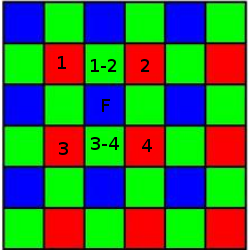
\includegraphics[scale=.3]{bayer1}}
	{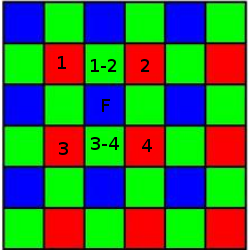
\includegraphics[scale=.3]{bayer1}}
	\caption{Direccional: rojos y azules} 
\end{figure}

Luego pasaremos a juntar ambas interpolaciones realizando otra interpolaci\'on m\'as, tomando los valores obtenidos anteriormente como los $y_{i}$, $x_{i}$ como los \textit{x} que se obtuvieron en cada interpolaci\'on (los cuales proven\'ian de un promedio) y \textit{x} como el promedio de estos dos puntos. Con este valor final hemos obtenido el valor del canal rojo para el pixel que estamos trabajando. A continuaci\'on se mostrar\'a un pseudoc\'odigo con los anteriormente explicado:

\hspace{5cm}

\begin{algorithm}[H]
Interpolar los puntos $(i-1,j-1)$ y $(i-1,j+1)$\\
Interpolar los puntos $(i+1,j-1)$ y $(i+1, j+1)$\\
Interpolar los resultados obtenidos anteriormente\\
Colocar resultado en canal rojo/azul del pixel (seg\'un corresponda)\\
\caption{Algoritmo para interpolar linealmente colores azules y rojos de pixel solo contiene componente verde}
\end{algorithm}
\hspace{5cm}

Luego de obtener el canal rojo y verde (este \'ultimo se explicar\'a en las pr\'oximas secciones), procederemos a buscar los canales azules y verdes para las filas que poseen solo colores rojos y verdes (filas impares) realizando exactamente lo mismo que anteriormente solo que seleccionaremos los canales rojos para interpolar en vez de los azules. Una vez realizado todo esto solo nos basta recorrer todos los p\'ixeles que poseen solo color verde para añadirles el canal rojo y azul. Para esto realizaremos una interpolaci\'on bilineal, la cual no explicaremos puesto que ya fue explicada anteriormente. De esta forma ya obtuvimos nuestra imagen final. 

A continuaci\'on presentaremos un algoritmo mostrando el esquema com\'un de las interpolaciones direccionales polin\'omicas:

\hspace{5cm}

\begin{algorithm}[H]
\textbf{IN} imagenBayer, \#filas, \#columnas \\
\textbf{OUT} imagen modificada\\
\For{Cada pixel azul de la imagen}{
	Canal verde en esa posicion = Aplicar algoritmo direccional saturando\\
	Realizar interpolacion bilineal sobre rojo \\
}
\For{Cada pixel rojo de la imagen}{
	Canal verde en esa posicion = Aplicar algoritmo direccional saturando\\
	Realizar interpolacion bilineal sobre azul \\
}
\For{Cada pixel verde de la imagen}{
	Canal rojo = Realizar interpolacion bilineal sobre rojo \\
	Canal azul = Realizar interpolacion bilineal sobre azul \\
}
\caption{Algoritmo Interpolaciones direccionales}
\end{algorithm}

\hspace{5cm}

\subsubsection{Direccional Diagonal 1}

Para este tipo de m\'etodo para resolver el problema de demosaicing hemos decidido realizar interpolaciones cruzadas de a 4 canales verdes a la vez para ver si es efectivo tomar tantos p\'ixeles en simult\'aneo (recordar que solo interpolaremos los verdes puesto que los rojos y azules ya fueron procesados). Este se encargar\'a de interpolar los canales verdes que rodean a aquellos p\'ixeles que solo poseen azul o rojo de la siguiente manera:

\begin{figure}[H]
\centering
	\subfigure[Direccional cruzado]{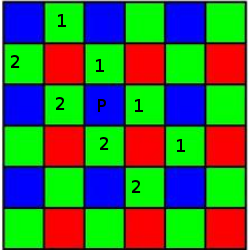
\includegraphics[scale=.35]{bayer2}}
	\subfigure[Direccional cruzado]{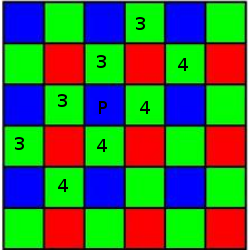
\includegraphics[scale=.35]{bayer3}}
	\caption{Direccional diagonal} 
\end{figure}

Para realizar el algoritmo, inicialmente interpolaremos los canales verdes de los 4 p\'ixeles que poseen el \'indice 1 en la figura mostrada anteriormente. Para realizar esta misma utilizaremos el polinomio de Lagrange mostrado antes, tomando como los $x_{i}$ la posici\'on que posee ese pixel dentro de la diagonal y como \textit{x} el promedio entre la posici\'on de los p\'ixeles en la diagonal que se encuentran en la primera y \'ultima posici\'on de la diagonal dentro de los seleccionados. Para hallar esta misma, utillizamos el siguiente algoritmo:

\vspace{0.5cm}

\begin{algorithm}[H]
\textbf{IN} fila actual del pixel(i), columna actual del pixel(j) \\
\textbf{OUT} posicion de la diagonal \\
	\eIf{i \textless $=j$}{
		return i\\
	}{
		return j\\
	}
\caption{Diagonal $\diagdown$}
\end{algorithm}

\vspace{0.5cm}

Este mismo se fija si el pixel buscado se encuentra sobre o debajo de la diagonal puesto que, dependiendo de esto, tendr\'a un valor distinto. Realizamos lo mismo para los p\'ixeles de \'indice 2. Una vez obtenidos estos dos valores, deberemos fusionarlos para as\'i obtener una estimaci\'on del canal verde en el pixel \textit{P} en esa direcci\'on. Para realizar esto, recurriendo al paper[2] (el cual indica que interpolar 2 valores es lo mismo que tomar el promedio entre ambos), hemos simplemente tomado el promedio de ambos. Con estos dos valores calculamos el gradiente que nos indicar\'a cu\'anto var\'ia el color verde entre esos dos puntos. Procedemos a realizar lo mismo para los \'indices 3 y 4 de la segunda imagen, teniendo en cuenta de que ahora el algoritmo para hallar en qu\'e posici\'on de la diagonal difiere ya que, al estar trabajando en otra direcci\'on, la primer diagonal con \'indice 0 se encontrar\'a al final del array de la imagen, siendo el siguiente:

\vspace{0.5cm}
\begin{algorithm}[H]
\textbf{IN} fila actual del pixel(i), columna actual del pixel(j), \# columnas imagen \\
\textbf{OUT} posicion de la diagonal \\
	\eIf{i \textgreater  $=columnas-j$}{
		return i\\
	}{
		return j\\
	}
\caption{Diagonal $\diagup$}
\end{algorithm}
\vspace{0.5cm}
Procedemos a calcular nuevamente el gradiente entre ambos para ver cu\'anto var\'ia el color verde y la estimaci\'on del canal verde del pixel \textit{P} en esa direcci\'on. Ahora solo resta unir estos valores hallados, teniendo en cuenta que hay que darle menos peso a la direcci\'on que posee un gradiente mayor, lo cual fue explicado en la introducci\'on de interpolaciones direccionales. Para esto recurrimos a la f\'ormula siguiente (siendo gradiente1 y gradiente2 los gradientes obtenidos anteriormente, y estx y esty los valores obtenidos sobre la estimaci\'on del canal verde del punto \textit{P}):

\begin{center}
$(255-gradiente1)/(2*255.0-gradiente1-gradiente2)*estx$\\$+$\\$(255-gradiente2)/(2*255.0-gradiente1-gradiente2)*esty$
\end{center}

Ahora solo resta saturar el valor obtenido para que se encuentra dentro del rango de los colores RGB y colocarlo en el canal verde del pixel seleccionado. De esta forma hemos obtenido el valor buscado. 

A continuaci\'on presentaremos un pseudoc\'odigo de lo anteriormente explicado:

%falta direccional 5 
\vspace{0.5cm}
\begin{algorithm}[H]
\textbf{IN} \textit{i,j} la posicion del pixel actual \\
\textbf{OUT} valor del verde en esa posicion\\
//Tomamos posicion en la diagonal como \textit{x} de la interpolacion\\
//Tomamos valor verde del pixel como \textit{y} de la interpolacion\\
\begin{enumerate}[label=\bfseries Step \arabic*:]
\item Interpolar los 4 pixeles diagonales superiores en direccion $\diagdown$: $(i-2,j-1),(i-1,j),(i,j+1),(i+1,j+2)$\\
\item Interpolar los 4 pixeles diagonales inferiores en direccion $\diagdown$: $(i-1, j-2),(i, j-1),(i+1, j),(i+2, j+1)$\\
\item Interpolar ambos resultados (tomando promedio)\\
\item \textit{gradiente1} = Gradiente entre ambas interpolaciones\\
\item Interpolar los 4 pixeles diagonales superiores en direccion $\diagup$: $(i-2, j+1),(i-1, j), (i, j-1), (i+1, j-2)$
\item Interpolar los 4 pixeles diagonales inferiores en direccion $\diagup$: $(i-1, j+2),(i, j+1), (i+1, j, (i+2, j-1)$
\item Interpolar ambos resultados (tomando promedio)\\
\item \textit{gradiente2} = Gradiente entre ambas interpolaciones\\
\item Unir interpolaciones tomando en cuenta los gradientes\\
\end{enumerate}
\caption{Direccional diagonal 1}
\end{algorithm}
\vspace{0.5cm}

\subsubsection{Direccional Horizontal y vertical}

Otra direcci\'on en la que hemos decidido interpolar para hallar el canal verde del pixel buscado es vertical y horizontalmente. \'Este tomar\'a los 3 p\'ixeles superior e inferior, y los 3 p\'ixeles a la izquierda y derecha, y los interpolar\'a. La siguiente figura muestra lo buscado:
\begin{figure}[H]
\centering
	%\subfigure[Direccional: rojos y azules]{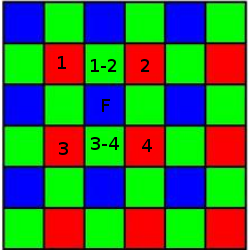
\includegraphics[scale=.3]{bayer1}}
	{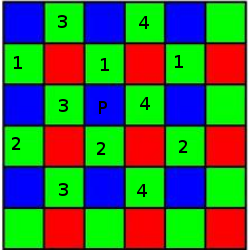
\includegraphics[scale=.3]{bayer4}}
	\caption{Direccional Vertical y horizontal} 
\end{figure}

Para la realizaci\'on del mismo procederemos como el anterior algoritmo direccional. Tomaremos los canales verdes de los 3 p\'ixeles que poseen el \'indice 1, 2, 3 y 4. Para el mismo utilizaremos el polinomio de Lagrange, del cual tomaremos como los $x_{i}$ la posici\'on que posee ese pixel dentro del array de la imagen y como \textit{x} el promedio entre la posici\'on del primer y \'ultimo pixel dentro de los seleccionados. Luego tomaremos el gradiente de los resultados obtenidos entre la interpolaci\'on entre los que ten\'ian \'indice 1 y 2, y luego los interpolaremos linealmente. Realizamos lo mismo para aquellos obtenidos a trav\'es de los que poseen el \'indice 3 y 4. Finalmente utilizamos la misma f\'ormula de pesos mostrada en el apartado anterior para unir todos estos canales verdes y colocaremos el resultado final en el pixel correspondiente (sin olvidarse de la saturaci\'on). 

A continuaci\'on se mostrar\'a un pseudoc\'odigo de lo anteriormente discutido:

\vspace{0.5cm}
\begin{algorithm}[H]
\textbf{IN} \textit{i,j} la posicion del pixel actual \\
\textbf{OUT} valor del verde en esa posicion\\
//Tomamos posicion en la matriz  como \textit{x} de la interpolacion\\
//Tomamos valor verde del pixel como \textit{y} de la interpolacion\\
\begin{enumerate}[label=\bfseries Step \arabic*:]
\item Interpolar los 3 pixeles inferiores: $(i-1,j-2),(i-1,j),(i-1,j+2)$\\
\item Interpolar los 3 pixeles superiores: $(i+1,j-2),(i+1,j),(i+1,j+2)$\\
\item Interpolar ambos resultados (tomando promedio)\\
\item \textit{gradiente1} = Gradiente entre ambas interpolaciones\\
\item Interpolar los 3 pixeles inferiores: $(i-2, j-1),(i, j-1), (i+2, j-1)$
\item Interpolar los 3 pixeles superiores: $(i-2, j+1),(i, j+1), (i+2, j+1)$
\item Interpolar ambos resultados (tomando promedio)\\
\item \textit{gradiente2} = Gradiente entre ambas interpolaciones\\
\item Unir interpolaciones tomando en cuenta los gradientes\\
\end{enumerate}
\caption{Direccional vertical y horizontal}
\end{algorithm}
\vspace{0.5cm}

\subsubsection{Direccional Combinada}

Para este m\'etodo queriamos fusionar los dos realizados anteriormente para evaluar qu\'e genera la uni\'on de todas estas interpolaciones. Para recordar los p\'ixeles seleccionados, se muestra la siguiente figura:

\begin{figure}[H]
\centering
	\subfigure[Direccional diagonal]{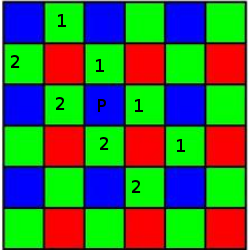
\includegraphics[scale=.3]{bayer2}}
	\subfigure[Direccional diagonal]{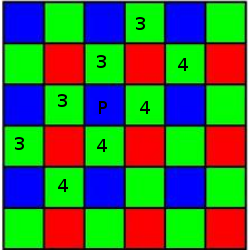
\includegraphics[scale=.3]{bayer3}}
	\subfigure[Direccional horizontal y vertical]{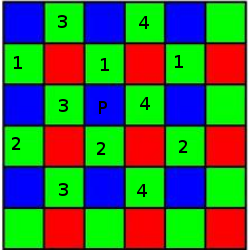
\includegraphics[scale=.3]{bayer4}}
	\caption{Direccionales combinados} 
\end{figure}

Para la realizaci\'on del mismo simplemente realizamos las mismas interpolaciones mostradas en los anteriores dos apartados, incluyendo la uni\'on de los mismos. La \'unica diferencia real entre los anteriores es que tuvimos que proceder a unir ambos resultados obtenidos, teniendo en cuenta todos los gradientes calculados, modificando un poco la f\'ormula utilizada anteriormente, cuyo resultado fue:

\begin{center}
$(255-((gradiente1 + gradiente2)/2))/(2*255.0-((gradiente1 + gradiente2)/2)-((gradiente3 + gradiente4)/2))*parcial1$\\
$+$\\
$(255-((gradiente3 + gradiente4)/2))/(2*255.0-((gradiente1 + gradiente2)/2)-((gradiente3 + gradiente4)/2))*parcial2;$
\end{center}

Siendo \textit{gradiente1, gradiente2} y \textit{parcial1} los resultados obtenidos con el algoritmo de direccionales diagonales, y \textit{gradiente3, gradiente4} y \textit{parcial2} los obtenidos en el de direccional horizontal y vertical. De esta forma obtuvimos el valor del canal verde del pixel seleccionado. 

A continuaci\'on presentaremos un algoritmo explicando lo anteriormente explicado:
%\vspace{0.5cm}

\begin{algorithm}[H]
\textbf{IN} \textit{i,j} la posicion del pixel actual \\
\textbf{OUT} valor del verde en esa posicion\\
//Tomamos posicion en la diagonal  como \textit{x} de la interpolacion\\
//Tomamos valor verde del pixel como \textit{y} de la interpolacion\\

\begin{enumerate}[label=\bfseries Step \arabic*:]
\item Interpolar los 4 pixeles diagonales superiores en direccion $\diagdown$: $(i-2,j-1),(i-1,j),(i,j+1),(i+1,j+2)$\\
\item Interpolar los 4 pixeles diagonales inferiores en direccion $\diagdown$: $(i-1, j-2),(i, j-1),(i+1, j),(i+2, j+1)$\\
\item Interpolar ambos resultados (tomando promedio)\\
\item \textit{gradiente3} = Gradiente entre ambas interpolaciones\\
\item Interpolar los 4 pixeles diagonales superiores en direccion $\diagup$: $(i-2, j+1),(i-1, j), (i, j-1), (i+1, j-2)$
\item Interpolar los 4 pixeles diagonales inferiores en direccion $\diagup$: $(i-1, j+2),(i, j+1), (i+1, j, (i+2, j-1)$
\item Interpolar ambos resultados (tomando promedio)\\
\item \textit{gradiente4} = Gradiente entre ambas interpolaciones\\
\item \textit{res1} = Unir interpolacion tomando en cuenta los gradientes\\
\end{enumerate}

//Tomamos posicion en la matriz  como \textit{x} de la interpolacion\\
//Tomamos valor verde del pixel como \textit{y} de la interpolacion\\

\begin{enumerate}[label=\bfseries Step \arabic*:]
\setcounter{enumi}{9}
\item Interpolar los 3 pixeles inferiores: $(i-1,j-2),(i-1,j),(i-1,j+2)$\\
\item Interpolar los 3 pixeles superiores: $(i+1,j-2),(i+1,j),(i+1,j+2)$\\
\item Interpolar ambos resultados (tomando promedio)\\
\item \textit{gradiente1} = Gradiente entre ambas interpolaciones\\
\item Interpolar los 3 pixeles inferiores: $(i-2, j-1),(i, j-1), (i+2, j-1)$
\item Interpolar los 3 pixeles superiores: $(i-2, j+1),(i, j+1), (i+2, j+1)$
\item Interpolar ambos resultados (tomando promedio)\\
\item \textit{gradiente2} = Gradiente entre ambas interpolaciones\\
\item \textit{res2} = Unir interpolacion tomando en cuenta los gradientes\\
Verde de imagen(i,j) = Unir \textit{res1} y \textit{res2} tomando en cuenta los gradientes \\
\end{enumerate}
\caption{Direccional combinada}
\end{algorithm}
\vspace{0.5cm}

\subsubsection{Direccional Diagonal 2}

Para realizar este tipo de interpolaci\'on direccional, hemos decidido realizar algo similar a la primera (diagonal) pero solamente tomando 3 p\'ixeles en vez de 4 a interpolar, como la siguiente imagen:

\begin{figure}[H]
\centering
	\subfigure[Direccional diagonal]{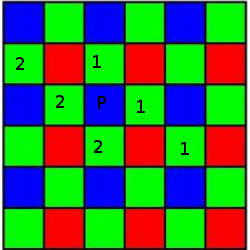
\includegraphics[scale=.35]{bayer5}}
	\subfigure[Direccional diagonal]{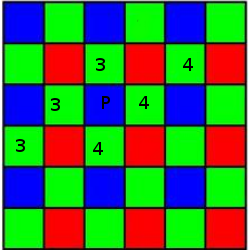
\includegraphics[scale=.35]{bayer6}}
	\caption{Direccional} 
\end{figure}

La misma proceder\'a de manera similar. Seleccionaremos de a 3 p\'ixeles como en la figura y los interpolaremos, tomando como $x_{i}$ la posici\'on que poseen en el array de la imagen. Una vez interpolados los canales verdes de los p\'ixeles que poseen el \'indice 1 y 2, tomaremos su gradiente e interpolaremos sus resultados a trav\'es de una interpolaci\'on lineal. Realizamos lo mismo para los que poseen \'indice 3 y 4. Para obtener el resultado utilizamos la misma f\'ormula que en el apartado de interpolaci\'on direccional diagonal 1 y saturamos. 

A continuaci\'on presentaremos un pseudoc\'odigo de lo anteriormente seleccionado:

\vspace{0.5cm}
\begin{algorithm}[H]
\textbf{IN} \textit{i,j} la posicion del pixel actual \\
\textbf{OUT} valor del verde en esa posicion\\
//Tomamos posicion en el array como \textit{x} de la interpolacion\\
//Tomamos valor verde del pixel como \textit{y} de la interpolacion\\
\begin{enumerate}[label=\bfseries Step \arabic*:]
\item Interpolar los 4 pixeles diagonales superiores en direccion $\diagdown$: $(i-1,j),(i,j+1),(i+1,j+2)$\\
\item Interpolar los 4 pixeles diagonales inferiores en direccion $\diagdown$: $(i-1,j-2),(i,j-1),(i+1,j)$\\
\item Interpolar ambos resultados con interpolaci\'on lineal\\
\item \textit{gradiente1} = Gradiente entre ambas interpolaciones\\
\item Interpolar los 4 pixeles diagonales superiores en direccion $\diagup$: $(i-1,j),(i,j-1),(i+1,j-2)$
\item Interpolar los 4 pixeles diagonales inferiores en direccion $\diagup$: $(i-1,j+2),(i,j+1),(i+1,j)$
\item Interpolar ambos resultados con interpolaci\'on lineal\\
\item \textit{gradiente2} = Gradiente entre ambas interpolaciones\\
\item Unir interpolaciones tomando en cuenta los gradientes\\
\end{enumerate}
\caption{Direccional diagonal 2}
\end{algorithm}
\vspace{0.5cm}

\subsection{Splines}

Uno de los primeros m\'etodos que implementamos para realizar esto fue la utilizaci\'on de interpolaci\'on por trazadores c\'ubicos (o tambi\'en llamados splines) para calcular dos estimaciones para cada canal verde de los pixeles que sea necesario. Es decir, para cada uno de estos punto calculamos el spline que pasa por su columna y fila y utilizamos estas funciones para estimar el valor que deber\'ia tener el canal verde evaluando las funciones estas en el valor que corresponda.
Con este fin, hicimos una funci\'on que dados $x_{i}$ y $f(x_{i})$ (i = 0,..n) calcula el trazador c\'ubico que pasa se obtiene con estos puntos, es decir busca $S(x)$ tal que:

\begin{enumerate}
\item S(x) es un polinomio de grado 3 ($S_{j}$) en [$x_{j}, x_{j+1}$] j=0,..,n-1
\item $S(x_{j})=f(x_{j}) j=0,..,n$
\item $S_{j}(x_{j+1}) = S_{j+1}(x_{j+1}) \ j=0,..,n-2$
\item $S_{j}'(x_{j+1}) = S_{j+1}'(x_{j+1}) \ j=0,..,n-2$
\item $S_{j}''(x_{j+1}) = S_{j+1}''(x_{j+1}) \ j=0,..,n-2$
\item $S''(x_{0}) = 0 \ y \ S''(x_{n}) = 0$
\end{enumerate}

Para la condici\'on 6 teniamos dos posibles alternativas para elegir, que sea un spline con frontera sujeta o con frontera libre (como finalmente decidimos hacer), pero como la primera de las dos ser\'ia pedir:

\begin{centering}
$S'(x_{0}) = f'(x_{0}) \ y \ S'(x_{n}) = f'(x_{n})$
\end{centering}

Es por ello que como no poseemos los valores de \textit{f'} para ninguno de esos puntos decidimos optar por la otra opcio\'on, de utilizar fronteras sujetas.
Como se puede observar en las condiciones impuestas sobre \textit{S}, esta quedara separada en \textit{$S_{j}$} (con j=0,..,n-1), siendo cada una de estas una funci\'on cuadr\'atica. Es por eso que para obtener \textit{S} es suficiente obtener los coeficientes $a_{j}, b_{j}, c_{j}$ y $d_{j}$ para cada $S_{j}(x)$ si es que escribimos a esta funci\'on de la siguiente forma:

\begin{centering}
$S_{j} = a_{j}+b_{j}(x-x_{j})+c_{j}(x-x_{j})^2+d_{j}(x-x_{j})^3$
\end{centering}

La raz\'on por la que expresamos la funci\'on de esta manera es que de esta forma se puede aprovechar m\'as facilmente de ciertas propiedades y valores de la derivada primera y segunda de esta funci\'on para asi llegar a un algoritmo para poder calcular cada uno de los $a_{j}, b_{j}, c_{j}$ y $d_{j}$ (con j=0,..,n-1). El algoritmo que utilizamos para calcularlas es el siguiente (algoritmo sacado del libro \textit{Numerical Analysis} de Richard L. Burden y J. Douglas Faires \footnote{Burden Richard L. and Faires J. Douglas. Numerical Analysis. Ninth Edition. P\'aginas 149-150}):

\begin{algorithm}[H]
INPUT: $n, x_{0},..,x_{n}, f(x_{0}),..,f(x_{n})$
OUTPUT: $a_{j}, b_{j}, c_{j}, d_{j} for j =0,..,n-1$
\For{i = 0..n-1}{
	$a_{i} = f(x_{i})$
}

\For{i = 0..n-1}{
	$h_{i} = x_{i+1}-x_{i}$
}
\For{i = 1..n-1}{
	$\alpha_{i} = \dfrac{3}{h_{i}}(a_{i+1}-a_{i})-\dfrac{3}{h_{i-1}}(a_{i}-a_{i-1})$
}
$l_{0} = 1$
$\mu_{0} = 0$
$z_{0} = 0$
\For{i = 1..n-1}{
	$l_{i} = 2(x_{i+1}-x_{i-1})-h_{i-1}\mu_{i-1}$
	$\mu_{i} = \dfrac{h_{i}}{l_{i}}$
	$z_{i} = \dfrac{(\alpha_{i}-h_{i-1}z_{i-1})}{l_{i}}$
}
$l_{n} = 1$
$z_{n} = 0$
$c_{n} = 0$
\For{j = n-1..0}{
	$c_{j} = z_{j}-\mu_{j}c_{j+1}$
	$b_{j} = \dfrac{a_{j+1}-a{j}}{h_{j}}-\dfrac{h_{j}(c_{j+1}+2c_{j})}{3}$
	$d_{j} = \dfrac{c_{j+1}-c_{j})}{3h_{j}}$
}
\caption{Algoritmo de calculo de un spline}
\end{algorithm}

Entonces, luego de la ejecuci\'on de este algoritmo obtendremos los $a_{j}, b_{j}, c_{j}$ y $d_{j}$ (j=0,..,n-1) para cada $S_{j}$, es decir que ya pudimos obtener la funci\'on \textit{S(x)}, la cual podremos usar para calcular las estimaciones para los \textit{x} distintos a los que utilizamos para calcular esta funci\'on.
Despu\'es de realizar esta funci\'on pasamos a implementar el filtro que utiliza trazadores c\'ubicos para pasar de una imagen que para cada pixel posea solo informaci\'on de un canal de color (estando estos ordenados de la forma descripta previamente) a una que en cada uno de estos posea informaci\'on de todos los canales. En este, utilizaremos splines para calcular dos estimaciones del valor de cada pixel en el que falte valores para el canal verde (una con la fila de la imagen y la otra con la columna), combinando luego ambas mediante una f\'ormula apropiada. La raz\'on por la que solo utilizamos los trazadores c\'ubicos para estimar los colores verdes es que para el ojo humano, de los 3 canales (rojo, azul y verde) este es el m\'as relevante, por lo que para los demas colores no es necesario obtener una estimaci\'on tan precisa. Con este fin, implementamos el siguiente algoritmo, el cual dada una imagen CFA Bayer devuelve una imagen RGB (Notaci\'on: $img_{x,y}[C]$, se refiere al valor del color C del pixel de la fila \textit{x} y columna \textit{y} de la imagen):

\begin{algorithm}[H]
INPUT: img (bayer array) \\
OUTPUT: sol (imagen RGB) \\
cantC = cantidad de columnas de la imagen \\
cantF = cantidad de filas de la imagen \\
ximp = [0, 2, 4,...] (de tamanio: (cantC/2+(1 si cantC es impar, 0 sino)) \\
xpar = [1, 3, 5,...] (de tamanio: (cantC/2)) \\
Matriz splFila; \\
\end{algorithm}
\begin{algorithm}[H]
\For{f = 1,..,cantF-1}{
	\If{f es par}{
		Calculamos Spline $F_{j}$
		Ponemos un 0 al final de $F_{j}$ de splFila \\
		\For{col = 0,..,tamanio de a-1}{
			Calculamos cuanto vale $S_{j}(ximp_{col+1})$ y lo guardamos al final de la $F_{j}$ de splFila \\
			Ponemos un 0 al final de $F_{j}$ de splFila \\
		}
		\If{cantC es par}{
			Sacamos el ultimo valor que colocamos en $F_{j}$ de splFila \\
		}
	}
	\Else{
		Calculamos Spline $F_{j}$
		\For{col = 0,..,tamanio de a-1}{
			Calculamos cuanto vale $S_{j}(ximp_{col})$ y lo guardamos al final de la $F_{j}$ de splFila \\
			Ponemos un 0 al final de $F_{j}$ de splFila \\
		}
		\If{cantC es impar}{
			Sacamos el ultimo valor que colocamos en $F_{j}$ de splFila \\
		}
	}
}
\end{algorithm}
\begin{algorithm}[H]
ximpC = [0, 2, 4,...] (de tamanio: (cantF/2+(1 si cantF es impar, 0 sino)) \\
xparC = [1, 3, 5,...] (de tamanio: (cantF/2)) \\
Matriz splCol; \\
\end{algorithm}
\begin{algorithm}[H]
\For{col = 1,..,cantC-1}{

	\If{col es par}{
		Calculamos Spline $C_{j}$
		Ponemos un 0 al final de $C_{j}$ de splFila \\
		\For{col = 0,..,tamanio de a-1}{
			Calculamos cuanto vale $S_{j}(ximp_{f+1})$ y lo guardamos al final de la $C_{j}$ de splFila \\
			Ponemos un 0 al final de $C_{j}$ de splFila \\
		}
		\If{cantF es par}{
			Sacamos el ultimo valor que colocamos en $C_{j}$ de splFila \\
		}
	}
	\Else{
		Calculamos Spline $C_{j}$
		\For{col = 0,..,tamanio de a-1}{
			Calculamos cuanto vale $S_{j}(ximp_{f})$ y lo guardamos al final de la $C_{j}$ de splFila \\
			Ponemos un 0 al final de $C_{j}$ de splFila \\
		}
		\If{cantF es impar}{
			Sacamos el ultimo valor que colocamos en $C_{j}$ de splFila \\
		}
	}
}
\end{algorithm}
\begin{algorithm}[H]
\For{f = 1,..,cantF-2}{
	\For{col = 1,..,cantC-2}{
		fsol = f-1 \\
		csol = c-1 \\
		\If{Estamos en un pixel verde}{
			\If{El pixel tiene rojo arriba y abajo}{
				$sol_{fsol, csol}[R] = \dfrac{img_{f-1,c}[R]+img_{f+1,c}[R]}{2}$ \\
				$sol_{fsol, csol}[G] = img_{f,c}[G]$ \\
				$sol_{fsol, csol}[B] = \dfrac{img_{f,c-1}[B]+img_{f,c+1}[B]}{2}$ \\
			}
			\Else{
				$sol_{fsol, csol}[R] = \dfrac{img_{f,c-1}[R]+img_{f,c+1}[R]}{2}$ \\
				$sol_{fsol, csol}[G] = img_{f,c}[G]$ \\
				$sol_{fsol, csol}[B] = \dfrac{img_{f-1,c}[B]+img_{f+1,c}[B]}{2}$ \\
			}
		}
		\Else{
			\If{Estamos en un pixel azul}{
				$sol_{fsol, csol}[R] = \dfrac{img_{f-1, c-1}[R]+img_{f-1, c+1}[R]+img_{f+1, c-1}[R]+img_{f+1, c+1}[R]}{4}$ \\
				$sol_{fsol, csol}[B] = img_{f, c}[B]$ \\
			}
			\Else{
				$sol_{fsol, csol}[R] = img_{f, c}[R]$ \\
				$sol_{fsol, csol}[B] = \dfrac{img_{f-1, c-1}[B]+img_{f-1, c+1}[B]+img_{f+1, c-1}[B]+img_{f+1, c+1}[B]}{4}$ \\
			}
			$GfilaEst = splFila_{fsol, csol}$ \\
			$GcolEst = splCol_{fsol, csol}$ \\
			$gradx = |img_{f,c-1}[G]-img{f,c+1}[G]|$ \\
			$grady = |img_{f-1,c}[G]-img{f+1,c}[G]|$ \\
			$sol_{fsol, csol}[G] = \dfrac{255-gradx}{255*2-gradx-grady}GfilaEst+\dfrac{255-grady}{255*2-gradx-grady}GcolEst$ \\
		}
	}
}
\caption{Algoritmo para la interpolacion usando splines}
\end{algorithm}

El objetivo de esta funci\'on es que para cada pixel en donde no hay informaci\'on del canal verde se haga una interporlaci\'on por trazadores c\'ubicos de la fila y de la columna, y luego combinar ambos valores con la ayuda del gradiente. Para la realizaci\'on de la interpolaci\'on de la fila, tomamos como los $x_{j}$ al n\'umero de columna de cada pixel (del que tenemos informaci\'on del canal verde), mientras que para la interpolaci\'on de la columna tomamos el n\'umero de la fila, tomando en ambos casos como $y_{j}$ el valor del canal verde en esos puntos. Entonces para buscar la estimaci\'on mediante splines de la fila y columna de un punto solo basta evaluar cada una de las \textit{S(x)} obtenidas con la fila y columna en su n\'umero de columna y fila respectivamente. Luego, estos valores los combinaremos dependiendo de como es el gradiente de los valores verdes horizontal y verticalmente, de forma tal que una estimaci\'on tenga mayor importancia si es que el gradiente en esa direcci\'on es menor. La raz\'on por la que juntamos los valores de esta forma es que un gradiente grande en una direcci\'on esta asociado con una variaci\'on grande del color, por lo que si hay un gradiente muy grande en general es porque ese punto se trata de un borde. Para estimar los gradientes en ambas direcciones utilizamos el m\'etodo de diferencias finitas de primer orden, lo que se traduce a que:

\begin{center}
$|\partial_{x}img_{x,y}[G]| \simeq |img_{x-1,y}[G]-img_{x+1,y}|$

$|\partial_{y}img_{x,y}[G]| \simeq |img_{x,y-1}[G]-img_{x,y+1}|$
\end{center}

Luego de obtener estos dos valores, juntamos estos valores junto con las estimaciones para poder otorgarle un \'unico valor al pixel del que estamos tratando de obtener una aproximaci\'on. Esto lo hacemos con la siguiente f\'ormula:

\begin{center}
$\dfrac{255-\partial_{x}img_{x,y}[G]}{255*2-\partial_{x}img_{x,y}[G]-\partial_{y}img_{x,y}[G]}estFila_{x,y}+\dfrac{255-\partial_{y}img_{x,y}[G]}{255*2-\partial_{x}img_{x,y}[G]-\partial_{y}img_{x,y}[G]}estCol_{x,y}$
\end{center}

Una de las principales razones por la que usamos esta f\'ormula es que satisface que cuanto mayor sea el gradiente en una direcci\'on, menor va a ser la importancia que le daremos a esa estimaci\'on, lo cual es \'util para que en caso de que haya un borde en una direcci\'on (porque en ese caso usariamos principalmente la otra estimaci\'on), adem\'as que se le otorga mayor peso a la estimaci\'on en cuya direcci\'on varia menos el color verde.
Con el objetivo de realizar lo descripto previamente para cada pixel donde falte el valor del canal verde, calculamos 2 matrices, una que posea las estimaciones por splines de cada columna y la otra por fila, conteniendo ambas 2 filas y columnas menos que la imagen. Esto se debe a que para la realizaci\'on de este algoritmo decidimos recortar los bordes de la imagen para no realizar estimaciones con splines de puntos que no tengan pixeles con valores verdes a ambos lados porque consideramos que estos podian poseer un mayor error que los otros (adem\'as de que como el recorte es m\'inimo apenas influye en la imagen). Adem\'as, esta matriz la llenamos con ceros en las posiciones en las cuales ya poseemos el valor del pixel verde en esa posici\'on, debido a que solo utilizaremos los otros valores pero es conveniente que el tamaño de la matriz sea este para un acceso m\'as intuitivo. Con el fin de obtener estas matrices, recorremos la imagen, calculando splines por cada columna en un caso y por cada fila en el otro, y adem\'as usando esto para estimar los valores de los canales verdes en cada uno de los puntos en donde no poseemos informaci\'on de este de la misma fila o columna. Luego, al ir guardando los valores en la matriz, al terminar el ciclo poseeremos de las dos matrices que deseamos y podemos usar los valores obtenidos para estimar el valor del color verde en nuestra imagen.
Entonces, en el \'ultimo ciclo recorremos la imagen, calculando las estimaciones de cada uno de los canales en los pixeles que haga falta, estimando los valores de los canales rojo y azul realizando un promedio de los puntos m\'as cercanos al que queremos estimar para ello y usando la f\'ormula de la que hablamos previamente para el caso del canal verde. La raz\'on por la cual tomamos diferentes indices para recorrer ambas im\'agenes es que la imagen \textit{sol} posee 2 filas y columnas menos (de igual forma de la que hacian las matrices con las estimaciones del canal verde), por lo que en $sol_{x,y}$ tiene que ir lo que deber\'ia ir en $img_{x-1, y-1}$
En conclusi\'on luego de terminar de ejecutar esta funci\'on llegamos a tener pasar de la imagen que en cada pixel solo tiene informaci\'on de un color a una que no, estimando los valores verdes que agregamos mediante una combinaci\'on de dos estimaciones realizadas mediante el c\'alculo de splines de la fila y la columna.

\section{Experimentos}
\subsection{Tiempo de Computo}

El objetivo de este experimento es evaluar los tiempos de c\'omputo de cada algoritmo en particular y luego realizar una comparaci\'on entre todos. Como trabajamos con procesamiento de im\'agenes, necesitamos que el tiempo que tardan en ejecutarse los algoritmos sea considerablemente buena, esto quiere decir que no tarde mucho puesto que hay un cliente esperando la imagen en RGB. 

Lo que se espera de este experimento es un poco predecible debido a c\'omo act\'uan nuestros algoritmos. Principalmente se sabe que, dependiendo del tamaño de la imagen, los algoritmos tomar\'an m\'as o menos tiempo, pero se busca evaluar cu\'anta diferencia hay entre estos. Adem\'as, esperamos que \textit{vecino m\'as cercano} sea el que menos tiempo lleve puesto que, para tomar el color de un canal que busca, solo toma el vecino por lo que no accede muchas veces a la imagen para obtener datos. Luego, como los algoritmos de Malvar, He cutler e interpolaci\'on bilineal se accede, por ciclo, no m\'as de tres veces a la imagen, esperamos que sean los siguientes en tardar menos, acompañado por splines. Por \'ultimo, como los direccionales acceden muchas veces a la imagen por ciclo puesto que interpolan en varias direccionaes simult\'aneamente, se espera que tengan un tiempo de c\'omputo elevado en comparaci\'on con los anteriores. 

Para medir los tiempos utilizamos la librer\'ia time.h. En particular la funci\'on clock. Esta devuelve el tiempo de procesador consumido por el programa. El valor devuelto se expresa en ciclos de reloj, que son unidades de tiempo de una longitud constante, pero específico del sistema (con una relación de $CLOCK-PER-SEC$ reloj ticks por segundo).

Con el fin de obtener una medida aceptable para los tiempos, tomaremos 10 mediciones y quitaremos las dos mayores y las dos menores para evitar los outliers. Despu\'es de eso, calculamos el promedio de las mediciones restantes. Para realizar una evaluaci\'on completa debemos, no solo analizar el tiempo de ejecuci\'on del algoritmo, sino tambi\'en  compararlo con muestras de distinto tamaño para poder observar como var\'ia respecto al tamaño de la matriz. 

En los siguientes gr\'aficos se puede ver los resultados con los distintos algoritmos de demosaicing:

\begin{figure}[H]
  \centering
    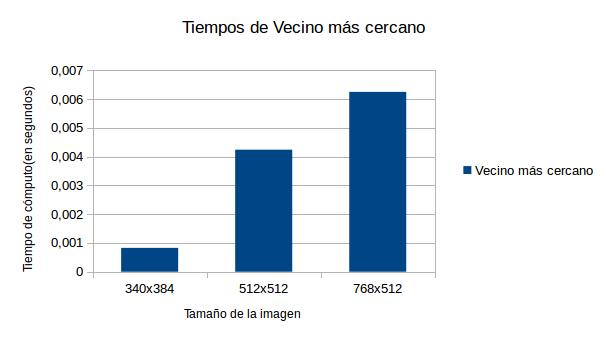
\includegraphics[width=0.9\textwidth]{vecino}
\end{figure}

\begin{figure}[H]
  \centering
    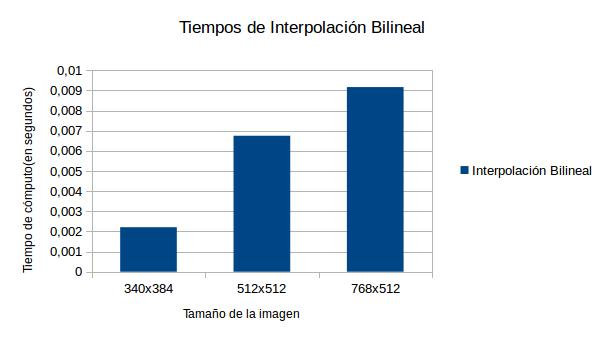
\includegraphics[width=0.9\textwidth]{Bilineal}
\end{figure}

\begin{figure}[H]
  \centering
    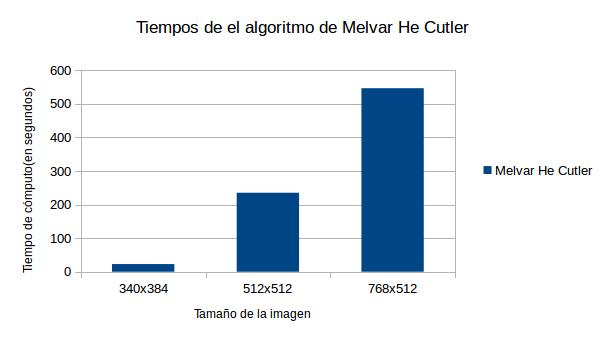
\includegraphics[width=0.9\textwidth]{MHC}
\end{figure}

\begin{figure}[H]
  \centering
    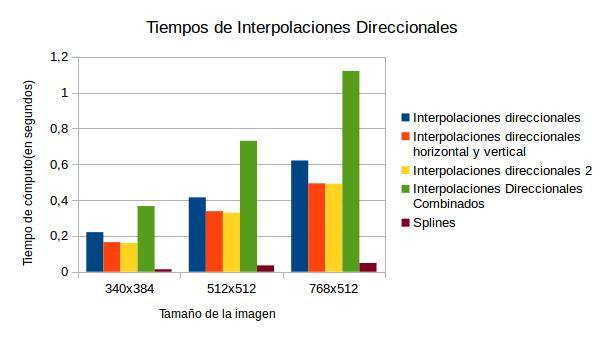
\includegraphics[width=0.9\textwidth]{Dir}
\end{figure}

Como podemos observar, para cada uno de los casos, el tiempo de c\'omputo es mayor en proporci\'on al tamaño de la imagen. Esto es normal porque en todos los algoritmos se realizan operaciones con los p\'ixeles recorriendo la matriz. Por lo tanto, entre m\'as grande sea esta, mayor ser\'a el n\'umero de operaciones a realizar. 

El principal objetivo de este experimento era averiguar cu\'al era el algoritmo m\'as r\'apido de todos porque estamos buscando el que sea mejor y, como estamos procesando im\'agenes, el tiempo de c\'omputo es importante. Para esto utilizaremos la informaci\'on obtenida en el test anterior sobre la imagen de mayor tamaño, juntando as\'i los resultados obtenidos. 

\begin{figure}[H]
  \centering
    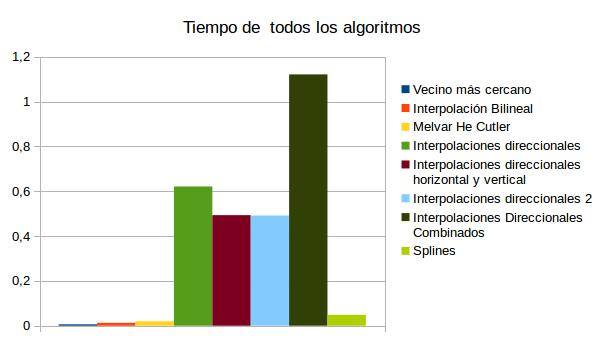
\includegraphics[width=0.9\textwidth]{Tiemp}
\end{figure}

En este gr\'afico podemos ver que los algoritmos con mejores tiempos son interpolaci\'on bilineal y vecino m\'as cercano. Esto es bastante l\'ogico porque estos son a su vez los m\'as simples, es decir que la cantidad de operaciones que se efect\'uan en ellos son pocas en comparaci\'on con las dem\'as, accediendo no tantas veces a la imagen para obtener los canales buscados. Despu\'es tenemos el algoritmo propuesto en [1] que solo implica usar bilineal y hacer una cantidad acotada de c\'alculos. Entre los algoritmos direccionales el que prevalece es el de splines el cual es considerablemente m\'as r\'apido respecto a los dem\'as de su mismo tipo. El peor de este tipo es el de super-direcciones puesto que combina dos direccionales que ya por separado tomaban bastante tiempo. 

En conclusi\'on, los tiempos de todos los algoritmos son bastante buenos (unos mejores que otros) para poder procesar im\'agenes en tiempo real. Ninguno se muestra como una mala alternativa en ese sentido, aunque en direccionales se pueden ver casos como super-direccionales y direccionales 1 que son definitivamente peores que los dem\'as en el sentido de tiempo de c\'omputo. 

\section{Calidad cuantificable}

El objetivo de este algoritmo es realizar un estudio de la calidad de las im\'agenes obtenidas a trav\'es de un m\'etodo llamado PSNR (Peak Signal-to-Noise Ratio), el cual compara los canales verdes de todos los p\'ixeles entre dos im\'agenes y nos devuelve un valor que indica que, entre mayor sea el mismo, m\'as parecida son las im\'agenes entre s\'i. 

Lo esperado de estos experimentos es que los algoritmos direccionales no posean un PSNR muy variado entre s\'i puesto que todos realizan algo similar en sus algoritmos, que a la vez son similares a bilineal. Vecino m\'as cercano no se espera que posea un PSNR  muy elevado, siendo peor que los anteriores, puesto que su m\'etodo es pobre ya que solo toma sus canales faltantes de los que se encuentran pr\'oximo a \'el. Respecto al propuesto en el Paper [1], se espera que sea el mejor de todos ya que este propone una mejora a interpolaciones bilineal y, como los direccionales se comportan de manera similar, luego Malvar deber\'ia ser mejor que todos ellos debido a los propuesto en dicho Paper. 
 
Para realizar este experimento calcularemos el PSNR para una imagen original y su versi\'on despu\'es de aplicarle alguno de nuestros algoritmos. Adem\'as, cortaremos los bordes de cada uno de manera sim\'etrica para asi poder comparar siempre los mismos p\'ixeles. Mostraremos los resultados obtenidos de las muestras propuestas por la c\'atedra: img1, img2, img4, img5 y img8. La raz\'on de dicha elecci\'on es que en estas se muestran problemas visualmente muy evidentes y adem\'as se repiten en casi todos los algoritmos, en menor y mayor medida. Mostraremos a continuaci\'on los resultados para cada una de las im\'agenes, recordando que entre mayor sea este, mejor ser\'a el filtro seg\'un.
\\
\indent
\begin{tabular}{| l | c | c | c | c | c |}
	\hline
	Imagen & Vecino más cercano	& Bilineal	&Splines	& Melvar He Cutler	&Direccional\\
img1	&30.854546	&35.927349	&27.929774	&40.28147	&36.216206	\\
img2	&24.042739	&28.233451	&21.816271	&32.649142	&28.459498	\\
img4	&23.328407	&26.55913	&18.438721	&31.056467	&26.920453	\\
img5	&28.154688	&32.851736	&24.730386	&37.16484	&33.169851	\\
img8	&27.962531	&33.684625	&23.57818	&38.201774	&34.669096	\\
	\hline
\end{tabular}
\\
\indent
\begin{tabular}{| l | c | c | c | c |}
	\hline
Imagen & Direccional horizontal y vertical	&Direccional Combinado	&Direccional 2\\
img1	&35.986055	&36.096432	&35.350906\\
img2	&28.326385	&28.381023	&26.692772\\
img4	&26.816371	&26.806714	&26.316806\\
img5	&32.983434	&33.051253	&32.017336\\
img8	&34.218966	&34.306257	&30.805319\\
	\hline
\end{tabular}
\\
Para poder evaluar su calidad de una manera simple, vamos a tomar el promedio de estos resultados para todos los algoritmos. Estos resultados se pueden observar en el siguiente gr\'afico:

\begin{figure}[H]
  \centering
    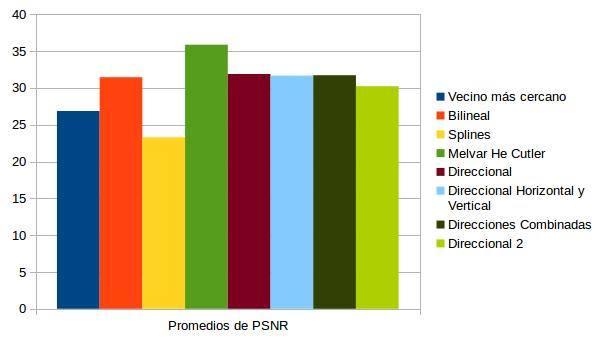
\includegraphics[width=0.9\textwidth]{PSNR}
\end{figure}

En la imagen se pudieron observar lo que esperaba de cada una de las im\'agenes. Se puede ver como el algoritmo de [1] termin\'o siendo el mejor, seguido de los direccionales polin\'omicos, interpolaciones bilineales, vecino m\'as cercano y splines. Si bien cada uno de ellos puede funcionar mejor o no dependendiendo del contexto de aplicaci\'on, se puede observar un estimativo de cuan bien o mal funcionan en general. Los direccionales polin\'omicos y bilineal tuvieron una perfomance muy similar, lo cual es normal ya que se diferencian en muy poco, lo cual la direcci\'on y/o la cantidad de p\'ixeles a interpolar. El m\'etodo propuesto de Malvar, He y Cutler para mejorar la interpolaci\'on bilineal termin\'o resultante muy buena, al menos respecto de los dem\'as algoritmos realizados. Finalmente, vecino m\'as cercanos y splines fueron los peores de todos, esto es debido a que el m\'etodo que utilizan para obtener los distintos canales no es muy efectivo ya que, por ejemplo en splines, no deber\'ia interesarnos los colores de toda una fila o columna para obtener el color del pixel actual. 

En conclusi\'on, este experimento cumpli\'o con nuestras expectativas iniciales. Pudimos observar c\'omo el PSNR de Malvar, He y Cutler fue el mejor de todos, mientras que los direccionales y bilineal fueron los siguientes y, por \'ultimo, vecino m\'as cercano y splines. Todo esto era esperado debido a la forma en la que estos algoritmos trabajaban. 

\section{Estudio subjetivo}

Para este experimento buscaremos realizar un an\'asis subjetivo de las im\'agenes obtenidos con los algoritmos propuestos. Buscaremos evaluar una serie de im\'agenes y buscar \textit{artifacts} en las mismas, que son errores que se encuentran en la imagen debido a problemas de los algoritmos de demosaicing. Hablaremos de lo que es frecuente para cada filtro y realizaremos comparaciones entre ellos. La idea de este experimento es ver si la imagen obtenido por los algoritmos es relativamente buena o no, puesto que somos las personas las que veremos dichas im\'agenes y podemos decidir, dada una imagen, cu\'al es su calidad. Ya que anteriormente se realizo el estudio de calidad cuantificable a trav\'es del PSNR, ya podemos hacernos una idea de c\'omo se ver\'a la imagen, solo basta revisarla para ver si coinciden dichos resultados con lo que el ojo humano ve. 

Para realizar el mismo hemos tomado todas las im\'agenes propuestas por la c\'atedra (12 en total) y aplicado cada uno de los algoritmos mencionados anteriormente en este informe. Hemos evaluado cada una de ellas y se hablar\'a de lo que se observ\'o en general para cada uno de ellos, realizando comparaciones. 

Al evaluar las im\'agenes obtenidas a trav\'es del algoritmo direccional diagonal que toma de a 4 p\'ixeles a la vez e interpola sus canales verdes, se pueden observar varios patrones entre ellos. Uno de los problemas que se encuentran es cuando hay objetos diagonales en la imagen como, por ejemplo, la soga de un barco. Esto es un problema puesto que se est\'a interpolando en ambas diagonales por lo que se mezcla lo que se encuentra en la diagonal que no est\'a en la imagen con la que s\'i. Esto provoca que aquellos objetos queden mal coloreados. Algo similar sucede en aquellos objetos que son finos puesto que tomamos 4 p\'ixeles para tomar su color verde y, si los objetos son muy finos, estaremos tomando cosas que no son de \'el, generando un color no deseado. Esto mismo se pudo observar en todas las im\'agenes evaluadas, notando que los colores obtenidos en esos p\'ixeles no est\'an bien respecto de la imagen. Debido a esto, cuando se encuentre un lugar de la imagen con bordes, estos no quedaran muy bien puesto que el rango de p\'ixeles seleccionados a interpolar es elevado, lo que genera una difuminaci\'on del color. Esto provoca que la imagen se encuentre borrosa respecto de la original. A continuaci\'on mostraremos algunos ejemplos en donde se pueden observar los hechos hablados anteriormente:

\begin{figure}[H]
\centering
	\subfigure[Artifacts]{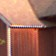
\includegraphics[scale=2.00]{1Subj6}}
	\subfigure[Artifacts]{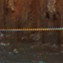
\includegraphics[scale=1.80]{1Subj5}}
	\subfigure[Artifacts]{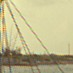
\includegraphics[scale=1.70]{1Subj4}}	
	\caption{Artifacts Direccional diagonal} 
\end{figure}


Cuando se eval\'ua el algoritmo direccional horizontal y vertical se pueden observar cosas similares al anterior. Una de las desventajas del mismo es que, al interpolar vertical y horizontalmente, luego en aquellos objetos diagonales no tendremos una buena estimaci\'on de su color ya que estamos estimando todo lo que est\'a a su alrededor, m\'as que el mismo. Esto mismo puede ser una ventaja a veces ya que hay objetos rectangulares/cuadrados que estima mejor ya que con uno diagonal podr\'iamos estar obteniendo valores fuera del mismo. Igualmente se encuentran \textit{artifacts} en todos los bordes u objetos finos, obteniendo p\'ixeles con coloraci\'on no deseada. A continuaci\'on mostraremos im\'agenes en las que se pueden observar las cosas mencionadas anteriormente, en donde se puede observar que la primer imagen obtuvo mejores resultados respecto de la primera del direccional anterior:

\begin{figure}[H]
\centering
	\subfigure[Artifacts]{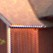
\includegraphics[scale=2.00]{2Subj7}}
	\subfigure[Artifacts]{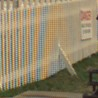
\includegraphics[scale=1.10]{2Subj8}}
	\subfigure[Artifacts]{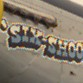
\includegraphics[scale=1.30]{2Subj9}}	
	\caption{Artifacts Direccional Horizontal y Vertical} 
\end{figure}

El algoritmo direccional combinado no difiere mucho de lo evaluado anteriormente puesto que es una combinaci\'on entre ambos, por lo que no se presentar\'an ejemplos. Si bien se tomaron en cuenta m\'as p\'ixeles a la hora de estimar sus valores, esto no tuvo un resultado muy exitoso ya que se puede observar en las im\'agenes que sigue habiendo problemas, que son los mismos que para los algoritmos mencionados antes. Esto se debe a que estamos seleccionando muchos p\'ixeles simult\'aneamente, lo que provoca que se mezclen demasiados grados de verde a la vez y no sea muy conciso al valor esperado. 

El algoritmo direccional diagonal que toma de a 3 p\'ixeles tuvo sus pro's y sus contra's al evaluar los resultados obtenidos. Tuvo mucha peor perfomance en algunas im\'agenes en comparaci\'on a lo obtenido con los anteriores, mientras que con otras im\'agenes tuvo resultados similares. Esto se pudo observar principalmente en la imagen siguiente:

\begin{figure}[H]
\centering
	%\subfigure[Direccional: rojos y azules]{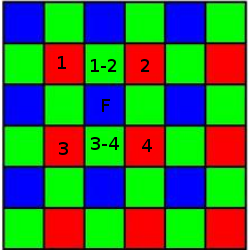
\includegraphics[scale=.3]{bayer1}}
	{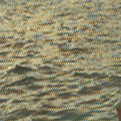
\includegraphics[scale=1.30]{5Subj2}}
	\caption{Artifacts Direccional 3} 
\end{figure}

Aqu\'i se puede notar c\'omo fue que quedaron los colores del agua. Dentro de los direccionales, ninguno tuvo un resultado similar a este. Esto se debe a que hab\'ian muchos bordes en los mismos y, como tomamos pocos p\'ixeles a la vez, quedo una mezcla indeseada. Una ventaja que se pudo observar respecto de los otros es que, en aquellos objetos diagonales, si bien no qued\'o con los colores deseados, no provoc\'o que el objeto perdiese su forma, como se pudo observar en las otras im\'agenes. Esto se puede ver en la siguiente imagen:

\begin{figure}[H]
\centering
	%\subfigure[Direccional: rojos y azules]{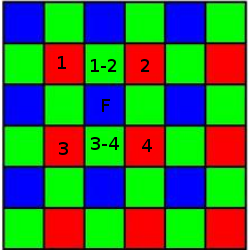
\includegraphics[scale=.3]{bayer1}}
	{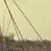
\includegraphics[scale=2.3]{5Subj3}}
	\caption{Artifacts Direccional 3} 
\end{figure}

Sin embargo, por lo que se puede observar, hubo im\'agenes que tuvieron resultados peores en algunos lugares, como se ver\'a en la p\'oxima imagen. En ninguna de las anteriores se pudo notar este problema en esta imagen, siendo esta la \'unica gener\'andolo. Se puede observar como no quedaron bien definidos los colores de las mismas. 

\begin{figure}[H]
\centering
	%\subfigure[Direccional: rojos y azules]{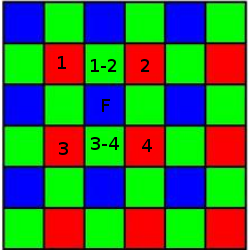
\includegraphics[scale=.3]{bayer1}}
	{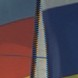
\includegraphics[scale=1.6]{5Subj1}}
	\caption{Artifacts Direccional 3} 
\end{figure}


En cuanto a los algoritmos direccionales, en todos se pudieron encontrar \textit{artifacts} similares, principalmente en los bordes, generando un efecto de \textit{zippering}. Esto gener\'o que no quedasen bien definido los colores de los mismos. Adem\'as se pudo observar en aquellos objetos finos algo similar ya que, al interpolar de varios p\'ixeles a la vez, se estaban tomando valores de otros objetos/fondo que no se deseaba. Otra cosa que se observo en todas las im\'agenes es que se encontraban difuminadas respecto de la original, esto es razonable debido a que al estar tomando de a varios p\'ixeles a la vez, se genera un desenfoque de la misma.  

Luego de los an\'alisis de los previos algoritmos, pasamos a analizar el funcionamiento del algoritmo de \textit{Splines}, con el fin de ver observar los resultados de este algoritmo y compararlo con las im\'agenes originales para ver que tan cercano esta su funcionamiento de lo esperado. Al igual que para los filtros realizados previamente, para realizar esto aplicamos esta funci\'on a las 12 im\'agenes que utilizamos para testear nuestros algoritmos, analizando lo ocurrido en todas ellas y mostrando los ejemplos de los problemas m\'as comunes.
Una de las primeras cosas que pudimos observar es que este algoritmo no es efectivo en la estimaci\'on del color de los bordes debido a que en la gran mayor\'ia de las im\'agenes se puede ver que en vez de haber los colores que deber\'ian, hay una mayor cantidad de rojo y azul. Esto es principalmente notorio en las sogas o bordes finos, en los cuales a veces ni se puede apreciar el verdadero color de estas debido a esa alteraci\'on, especialmente donde hay muchos bordes cercanos. Esto se puede ver por ejemplo en las siguientes im\'agenes, en las que se ve que en algunos pixeles el color de estos es muy ampliamente distinto del que tienen en la imagen original:
\begin{figure}[H]
\centering
	\subfigure[Artifacts]{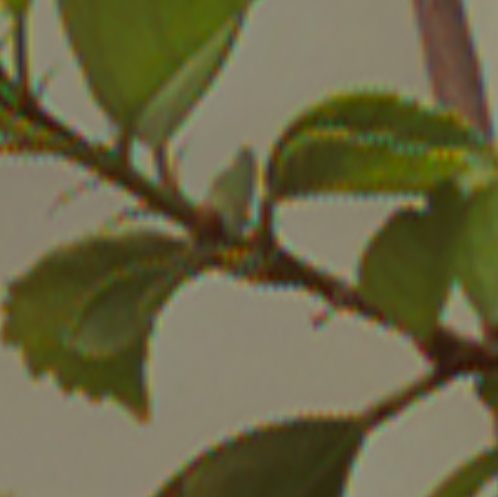
\includegraphics[scale=0.3]{Spl1}}
	\subfigure[Artifacts]{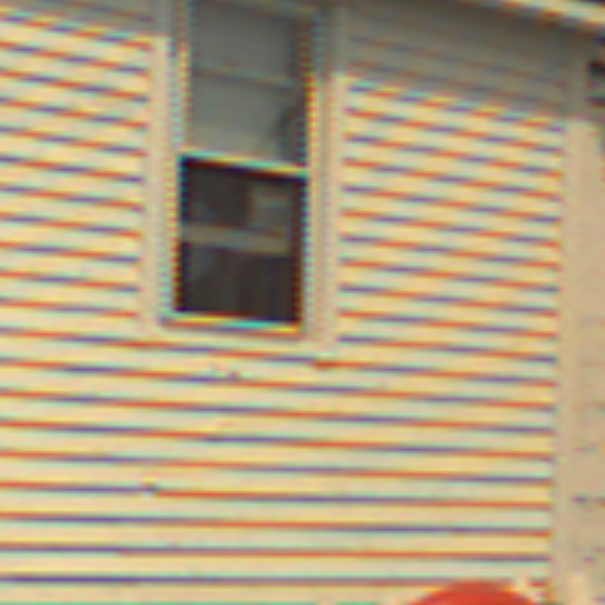
\includegraphics[scale=0.25]{Spl2}}
	\caption{Artifacts Splines (Bordes)} 
\end{figure}

Adem\'as, otro de los problemas que tiene la utilizaci\'on de splines, es que en casi todas las im\'agenes que contienen agua, el color de esta se ve distorsionado, con pixeles m\'as rojos o azules de lo que deber\'ian, siendo el mejor ejemplo de esto las im\'agenes mostradas a continuaci\'on, en las cual se puede ver a simple vista lo mencionado anteriormente:
\begin{figure}[H]
\centering
	\subfigure[Artifacts]{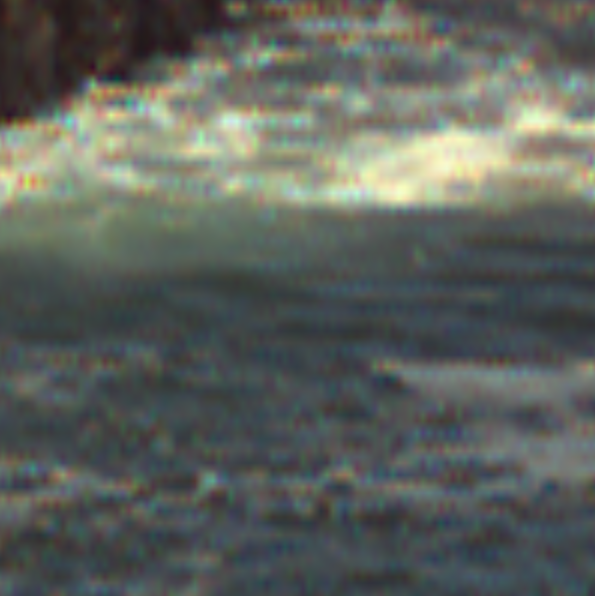
\includegraphics[scale=0.25]{Spl3}}	
	\caption{Artifacts Splines (Agua)} 
\end{figure}
Una de las principales fallas de este algoritmo (que suponemos que debe de causar muchos de los problemas mencionados anteriormente), es que solo considera estimaciones realizadas horizontal y verticalmente, por lo que esto puede ocasionar que el valor obtenido para un pixel mediante nuestro algoritmo no sea el que deba ser debido a que no se tomaron en cuenta una mayor cantidad de direcciones (o por ejemplo la realizaci\'on de estimaciones con diagonales).
En conclusi\'on el algoritmo de splines que implementamos no cumple muy efectivamente su funci\'on, debido a que tiene graves problemas para estimar el valor de cada uno de los canales de los pixeles en muchas ocasiones que son frecuentes al tomar fotograf\'ias. Estas situaciones son, por ejemplo, el caso en que haya agua o bordes, especialmente cuando se encuentran muchos de estos muy cercano, lo cual ocurre muy frecuentemente en las fotografias.

Pasamos luego a analizar que es lo que ocurr\'ia con el algoritmo \textit{Vecino m\'as cercano}, analizando las im\'agenes obtenidas de la misma manera que con los otros algoritmos, observando con detalle como son las im\'agenes obtenidas a partir de este algoritmo, buscando problemas, ocasiones en la que funciona correctamente y artifacts.
Uno de los primero problemas que se puede observar es que la imagen obtenida mediante este m\'etodo se ve pixelada y borrosa, hecho que muchas veces se puede observar muy a simple vista sin ser necesario observar con mucho detalle la imagen. Esto ocurre principalmente debido a que este algoritmo tiene muchos problemas para que la imagen quede correcta en los bordes, siendo esto muy claro en muchas ocasiones, habiendo casos en los que se ven pixeles rojos, azules y verdes distintos de los que lo rodean. Esto lo podemos observar muy claramente en las siguientes im\'agenes, en la cual no solo las im\'agenes se ven pixeladas, sino que tambi\'en se ve el efecto que provoca este m\'etodo en sus bordes:

\begin{figure}[H]
\centering
	\subfigure[Artifacts]{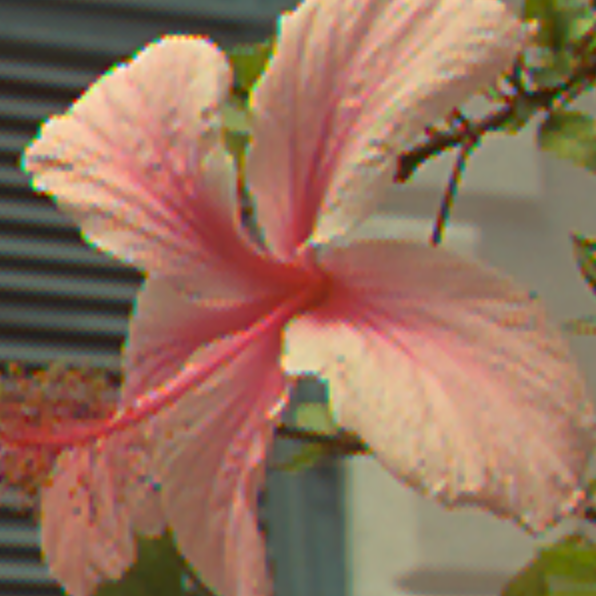
\includegraphics[scale=0.24]{VC1}}
	\subfigure[Artifacts]{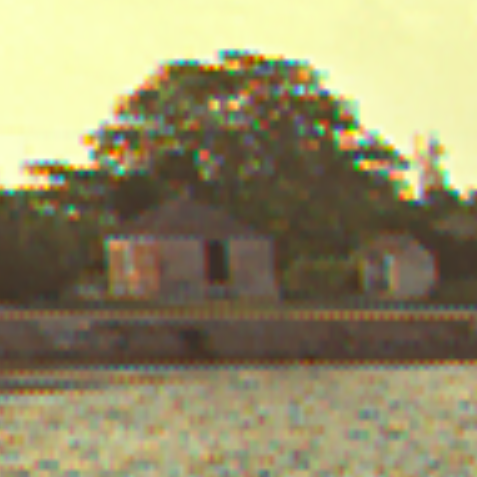
\includegraphics[scale=0.3]{VC2}}
	\subfigure[Artifacts]{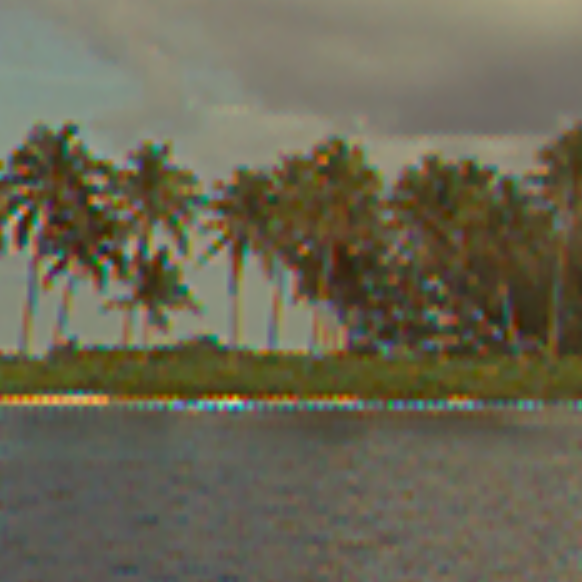
\includegraphics[scale=0.25]{VC3}}
	\caption{Artifacts Vecino m\'as cercano (Bordes)} 
\end{figure}

Algo tambi\'en importante a notar es que la utilizaci\'on de este m\'etodo provoca que el agua no este con la coloraci\'on adecuada, teniendo muchas veces pixeles con un color muy diferente del adecuado. Esto se puede observar en las siguientes im\'agenes:

\begin{figure}[H]
\centering
	\subfigure[Artifacts]{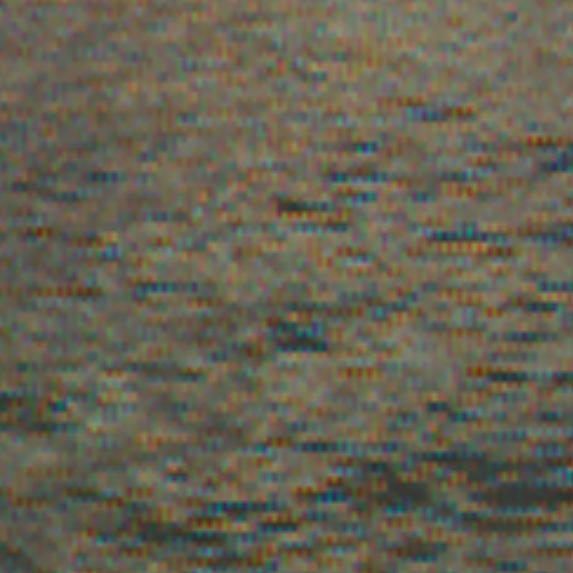
\includegraphics[scale=0.25]{VC4}}
	\subfigure[Artifacts]{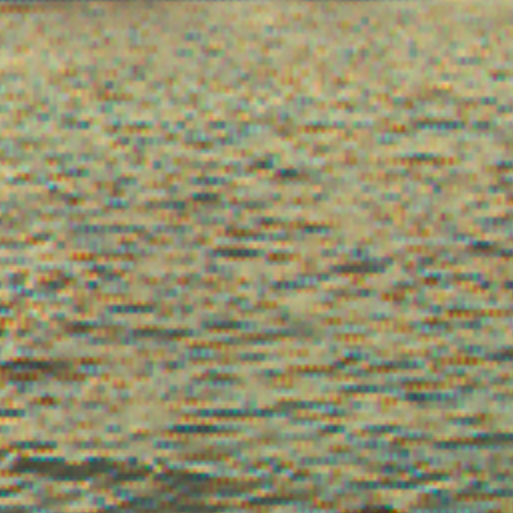
\includegraphics[scale=0.28]{VC5}}
	\caption{Artifacts Vecino m\'as cercano (Agua)} 
\end{figure}

Es por estas razones que no es conveniente la utilizaci\'on de este algoritmo para demosaicing debido a que las im\'agenes obtenidas mediante este m\'etodo son muy diferentes de las im\'agenes originales.

Continuamos luego analizando el funcionamiento del m\'etodo para pasar de una \textit{CFA Bayer} a una imagen \textit{RGB} utilizando el algoritmo de \textit{interpolaci\'on bilineal}, para lo cual aplicamos la funci\'on implementada a cada una de las 12 im\'agenes provistas por la c\'atedra. Al observar las im\'agenes generadas mediante este proceso, vimos que en muchas de estas ocurr\'ian similares problemas que en muchos de los algoritmos realizados por nosotros, principalmente, que la utilizaci\'on de este generaba un problema con los bordes en las im\'agenes. Esto se deb\'ia a que en muchos casos en los bordes hab\'ia problemas en la coloraci\'on de estos siendo distintos los colores de los originales. Esto se puede ver con mucha claridad en las siguientes im\'agenes:

\begin{figure}[H]
\centering
	\subfigure[Artifacts]{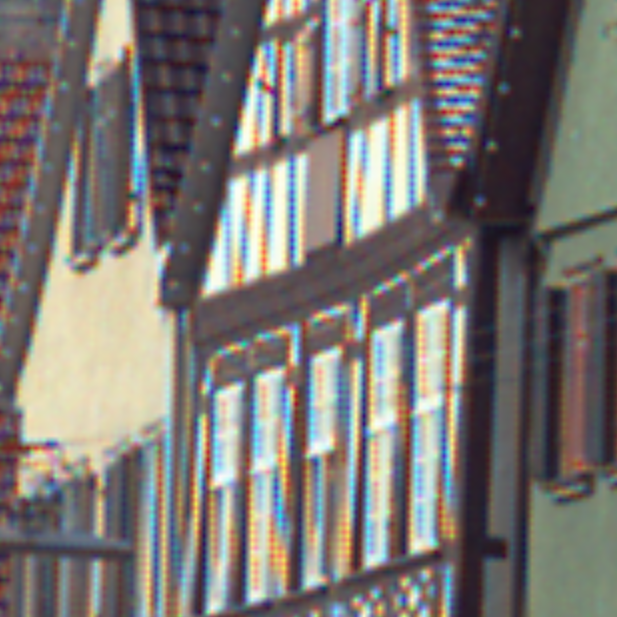
\includegraphics[scale=0.25]{Bi1}}
	\subfigure[Artifacts]{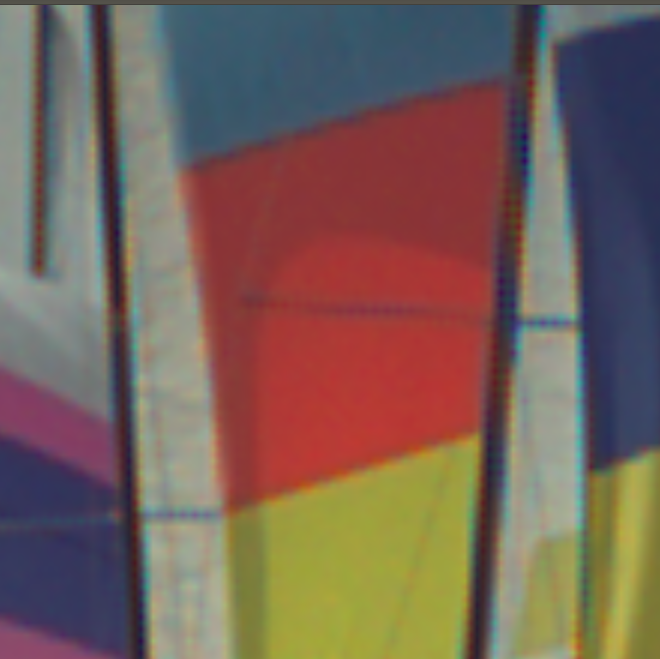
\includegraphics[scale=0.235]{Bi2}}
	\caption{Artifacts interpolaci\'on bilineal (Bordes)} 
\end{figure}

Aparte, otro de los problemas que ten\'ia nuestro algoritmo es que tambi\'en ten\'ia fallos al realizar las estimaciones de zonas de agua, lo cual se puede ver muy f\'acilmente en las siguiente im\'agenes:

\begin{figure}[H]
\centering
	\subfigure[Artifacts]{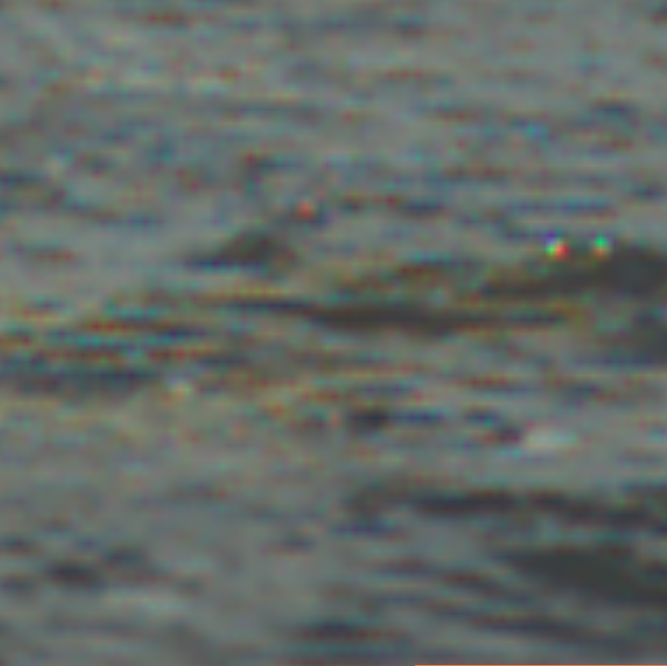
\includegraphics[scale=0.23]{Bi3}}
	\caption{Artifacts interpolaci\'on bilineal (Agua)} 
\end{figure}

Al evaluar lo que sucede con el algoritmo de \textit{Malvar, He y Cutler}, vimos que segu\'ian ocurriendo casi los mismos problemas que para los dem\'as m\'etodos, habiendo muchos casos en los que los que hay problemas con los bordes de las im\'agenes, principalmente en los casos que se traten de lineas finas como por ejemplo sucede con las sogas. Esto se puede ver por ejemplo en las siguientes im\'agenes:

\begin{figure}[H]
\centering
	\subfigure[Artifacts]{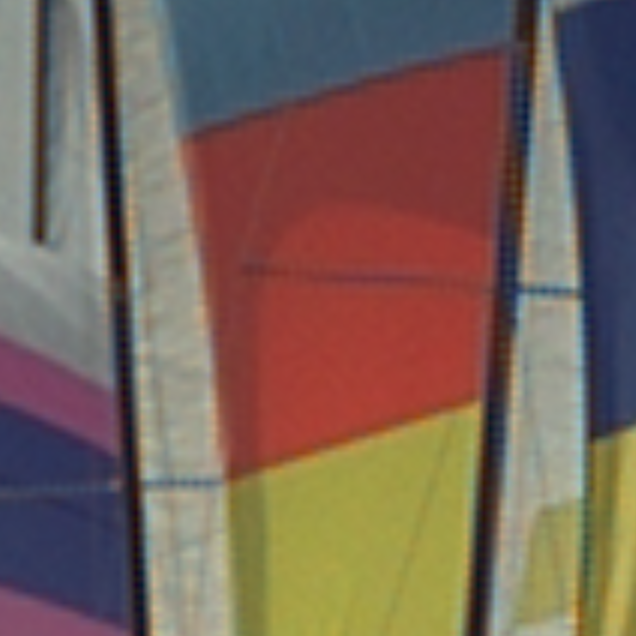
\includegraphics[scale=0.23]{Mal1}}
	\subfigure[Artifacts]{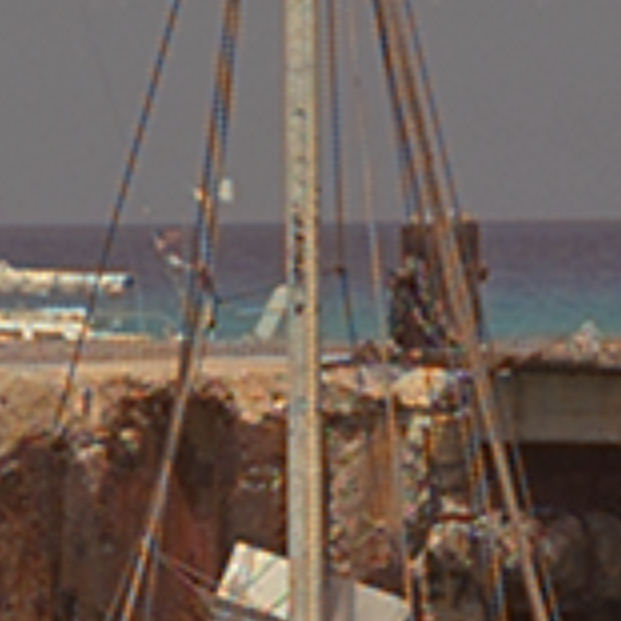
\includegraphics[scale=0.235]{Mal2}}
	\caption{Artifacts algoritmo de Malvar, He y Cutler (Bordes)} 
\end{figure}

Por otro lado, tambi\'en hay algunos problemas con este algoritmo cuando lo aplicamos a im\'agenes con mucha agua, en donde el color del agua no queda igual que en la imagen original, lo cual se puede ver por ejemplo en la siguiente imagen:

\begin{figure}[H]
\centering
	\subfigure[Artifacts]{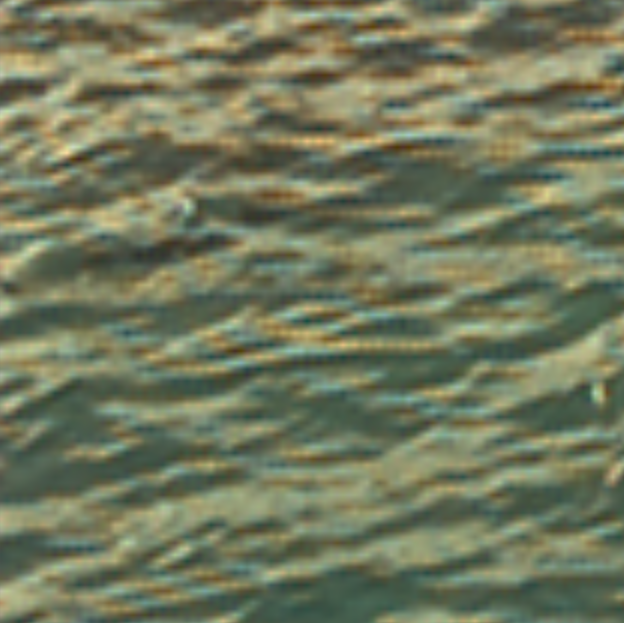
\includegraphics[scale=0.25]{Mal3}}
	\caption{Artifacts algoritmo de Malvar, He y Cutler (Agua)} 
\end{figure}

Pese a los problemas que tiene el uso de este algoritmo, este tambi\'en tiene muchos beneficios debido a que, a pesar de que muchos de los problemas que tenemos con otros m\'etodos siguen persistiendo, estos no son tan marcados como con los otros algoritmos y adem\'as hay algunas im\'agenes en las que con otros aparec\'ian pero utilizando el algoritmo de Malvar, He y Cutler.

Como conclusi\'on, vimos que los problemas en los algoritmos que realizamos para pasar de la imagen CFA Bayer a RGB son en general siempre los mismos, habiendo siempre problemas con los bordes y con el agua, aunque variando este en intensidad seg\'un el algoritmo que usamos. Por ejemplo, pudimos observar que en la mayor\'ia de las im\'agenes los filtros \textit{Vecino m\'as cercano} y \textit{Splines} resultaron en peores resultados, mientras que con los algoritmos \textit{Direccional}, \textit{Bilineal} y \textit{Malvar, He y Cutler} se obtuvieron las mejores im\'agenes, siendo especialmente eficiente el algoritmo de \textit{Malvar, He y Cutler} en casi todas las im\'agenes. Es por ello que de estos m\'etodos recomendamos utilizar el algoritmo de \textit{Malvar, He y Cutler} para realizar el demosaicing, por lo menos respecto a como se ve subjetivamente la imagen.
\section{Bibliograf\'ia}

\begin{thebibliography}{5}

\bibitem{MHC}
  Henrique S. Malvar, Li-wei He, and Ross Cutler,
  \emph{HIGH-QUALITY LINEAR INTERPOLATION FOR DEMOSAICING OF BAYER-PATTERNED COLOR IMAGES}.
  
\end{thebibliography}

\end{document}

\end{document}
